%,%%%%%%%%%%%%%%%%%%%%%%%%%%%%%%%%%%%%%%%%%%%%%%%%%%%%%%
% Please note that whilst this template provides a
% preview of the typeset manuscript for submission, it
% will not necessarily be the final publication layout.
%
% letterpaper/a4paper: US/UK paper size toggle
% num-refs/alpha-refs: numeric/author-year citation and bibliography toggle

%\documentclass[letterpaper]{oup-contemporary}
\documentclass[a4paper,num-refs]{oup-contemporary}

%%% Journal toggle; only specific options recognised.
%%% (Only "gigascience" and "general" are implemented now. Support for other journals is planned.)
\journal{preprint}

\usepackage{graphicx}
\usepackage{siunitx}
\usepackage[switch]{lineno}

\linenumbers

% Additional packages for data model figure
\usepackage{forest}
\usepackage{tikz}
\usetikzlibrary{quotes,arrows.meta,3d}

%%% Flushend: You can add this package to automatically balance the final page, but if things go awry (e.g. section contents appearing out-of-order or entire blocks or paragraphs are coloured), remove it!
% \usepackage{flushend}

% Macros etc for data model figure
\input{diagrams/data-model-preamble.tex}

% See https://github.com/sgkit-dev/vcf-zarr-publication/issues/87
% for discussion
\title{Analysis-ready VCF at Biobank scale using Zarr}

%%% Use the \authfn to add symbols for additional footnotes, if any.
% 1 is reserved for correspondence emails; then continuing with 2 etc for contributions.
% First author
\author[1,2\authfn{1}]{Eric Czech} % https://orcid.org/0000-0002-4254-4255
\author[3,4\authfn{1}]{Timothy R. Millar} % https://orcid.org/0000-0002-5142-8811
\author[5,\authfn{1}]{Will Tyler}
\author[6,\authfn{1}]{Tom White}

% Middle, alphabetical order
\author[7]{Benjamin Elsworth} % https://orcid.org/0000-0001-7328-4233
\author[8,9]{Jérémy Guez} % https://orcid.org/0009-0007-6406-5187
\author[10]{Jonny Hancox} % https://orcid.org/0009-0003-5799-5299
\author[11]{Ben Jeffery} % https://orcid.org/0000-0002-1982-6801
\author[8,9,12]{ Konrad J. Karczewski} % https://orcid.org/0000-0003-2878-4671
\author[13]{Alistair Miles} % https://orcid.org/0000-0001-9018-4680
\author[14]{Sam Tallman} % https://orcid.org/0000-0001-7183-6276
\author[15]{Per Unneberg} % https://orcid.org/0000-0001-5735-3315
\author[1]{Rafal Wojdyla} % https://orcid.org/0009-0005-0735-7090
\author[16]{Shadi Zabad} % https://orcid.org/0000-0002-8003-9284

% Senior
\author[1,2,\authfn{2}]{Jeff Hammerbacher} % https://orcid.org/0000-0001-6596-8563
\author[11,\authfn{2},\authfn{3}]{Jerome Kelleher} % https://orcid.org/0000-0002-7894-5253

\affil[1]{Open Athena AI Foundation}
\affil[2]{Related Sciences}
\affil[3]{The New Zealand Institute for Plant \& Food Research Ltd, Lincoln,
New Zealand}
\affil[4]{Department of Biochemistry, School of Biomedical Sciences, University of Otago, Dunedin, New Zealand}
\affil[5]{Independent researcher}
\affil[6]{Tom White Consulting Ltd.}
\affil[7]{Our Future Health, Manchester, UK.}
\affil[8]{Program in Medical and Population Genetics, Broad Institute of MIT and Harvard, Cambridge, Massachusetts 02142, USA}
\affil[9]{Analytic and Translational Genetics Unit, Massachusetts General
Hospital, Boston, Massachusetts 02114, USA}
\affil[10]{NVIDIA Ltd, Reading, UK}
\affil[11]{Big Data Institute, Li Ka Shing Centre for Health Information and Discovery,
University of Oxford, UK}
\affil[12]{Novo Nordisk Foundation Center for Genomic Mechanisms of Disease, Broad Institute of MIT and Harvard, Cambridge, Massachusetts 02142, USA}
\affil[13]{Wellcome Sanger Institute}
\affil[14]{Genomics England}
\affil[15]{Department of Cell and Molecular Biology, National
  Bioinformatics Infrastructure Sweden, Science for Life Laboratory,
  Uppsala University, Uppsala, Sweden}
\affil[16]{School of Computer Science, McGill University, Montreal, QC, Canada}

%%% Author Notes
\authnote{\authfn{1}Joint first author.}
\authnote{\authfn{2}Joint senior author.}
\authnote{\authfn{3}jerome.kelleher@bdi.ox.ac.uk}

%%% Paper category
\papercat{Paper}

%%% "Short" author for running page header
\runningauthor{Czech et al.}

%%% Should only be set by an editor
\jvolume{00}
\jnumber{0}
\jyear{2024}

\begin{document}

\begin{frontmatter}
\maketitle

% The Abstract (250 words maximum) should be structured to
% include the following details:
% \textbf{Background}, the context and purpose of
% the study;
% \textbf{Results}, the main findings;
% \textbf{Conclusions}, brief
% summary and potential implications. Please minimize the use of abbreviations
% and do not cite references in the abstract.
% The Abstract (250 words maximum) should be structured to
% include the following details:
% \textbf{Background}, the context and purpose of % the study;
% \textbf{Results}, the main findings;
% \textbf{Conclusions}, brief summary and potential implications.

%% NOTE: this is much too long currently, but keeping for now so we
% can see which stuff migrates to the intro
\begin{abstract}
\textbf{Background:}
Variant Call Format (VCF) is the standard file format for interchanging
genetic variation data and associated quality control metrics.
The usual row-wise encoding of the VCF data model (either as text
or packed binary) emphasises efficient retrieval of all data for a given
variant, but accessing data on a field or sample basis is inefficient.
Biobank scale datasets currently available
consist of hundreds of thousands of whole genomes
and hundreds of terabytes of compressed VCF.
Row-wise data storage is fundamentally unsuitable
and a more scalable approach is needed.

\textbf{Results:}
Zarr is a format for storing
multi-dimensional data that is widely used across the sciences,
and is ideally suited to massively parallel processing.
We present the VCF Zarr specification, an encoding of the
VCF data model using Zarr, along with fundamental software infrastructure
for efficient and reliable conversion at scale.
We show how this format is far more efficient than
standard VCF based approaches,
and competitive with specialised methods for
storing genotype data in terms of compression ratios
and single-threaded calculation performance.
We present case studies on subsets of three large 
human datasets (Genomics England: $n$=78,195;
Our Future Health: $n$=651,050; 
All of Us: $n$=245,394) along with whole genome
datasets for Norway Spruce ($n$=1,063) and 
SARS-CoV-2 ($n$=4,384,310), 
demonstrating the scalability and flexibility of VCF Zarr.
We demonstrate the potential for VCF Zarr to enable a new generation
of high-performance and cost-effective applications
via illustrative highly parallel benchmarks on AWS and experimentation with GPUs.

\textbf{Conclusions:}
Large row-encoded VCF files are a major bottleneck for current research, and
storing and processing these files incurs a substantial cost.
The VCF Zarr specification, building on widely-used, open-source technologies
has the potential to greatly reduce these costs,
and may enable a diverse ecosystem of next-generation tools for analysing
genetic variation data directly from cloud-based object stores,
while maintaining compatibility with existing file-oriented workflows.
\end{abstract}

\begin{keywords}
Variant Call Format; Zarr; Analysis ready data.
\end{keywords}
\end{frontmatter}

%%% Key points will be printed at top of second page
\begin{keypoints*}
\begin{itemize}
\item VCF is widely supported, and the underlying data model entrenched
in bioinformatics pipelines.
\item The standard row-wise encoding as text (or binary) is inherently
inefficient for large-scale data processing.
\item The Zarr format provides an efficient solution, by encoding fields
in the VCF separately in chunk-compressed binary format.
\end{itemize}
\end{keypoints*}

\section{Background}
Variant Call Format (VCF) is the standard format for interchanging genetic
variation data, encoding information about
DNA sequence polymorphisms among a set of samples with associated
quality control metrics and metadata~\citep{danecek2011variant}.
Originally defined specifically as a text file,
it has been refined and standardised~\citep{rehm2021ga4gh} and the
underlying data-model is now deeply embedded in bioinformatics practice.
Dataset sizes have grown explosively since the introduction of
VCF as part of 1000 Genomes project~\citep{10002015global},
with Biobank scale initiatives such as
Genomics England~\cite{turnbull2018100},
UK Biobank~\citep{bycroft2018genome,backman2021exome,halldorsson2022sequences,uk2023whole},
Our Future Health~\citep{cook2025our,ofhmain_2025},
and the All of Us research program~\citep{all2024genomic}
collecting genome sequence data for millions of humans~\citep{stark2024call}.
Large genetic variation datasets are also being generated for other organisms
and a variety of purposes including
agriculture~\citep{ros2020accuracy,wang2023rice},
conservation~\citep{shaffer2022landscape}
and infectious disease surveillance~\citep{hamid2023pf7}.
VCF's simple text-based design and widespread
support~\cite{garrison2022spectrum} make it an
excellent archival format, but it is an inefficient basis for analysis.
Methods that require efficient access to genotype data
either require conversion to the
PLINK~\cite{purcell2007plink,chang2015second}
or BGEN~\citep{band2018bgen}
formats~\citep[e.g.][]{yang2011gcta,mbatchou2021computationally,loh2015efficient}
or use bespoke binary formats
that support the required access patterns~\citep[e.g.][]{
% Uses custom "bref3" format,
% https://faculty.washington.edu/browning/beagle/bref3.24May18.pdf
browning2018one,
% .samples Zarr format
kelleher2019inferring,
% Has a "xcftools" package, but it still looks pretty experimental
hofmeister2023accurate}.
While PLINK and BGEN formats are more efficient to access than VCF, neither
can accommodate the full flexibility of the VCF data model and conversion
is lossy.
PLINK's approach of storing the genotype matrix in uncompressed
packed-binary format provides efficient access to genotype
data, but file sizes are substantially larger than
the equivalent compressed VCF (see Fig~\ref{fig-data-storage}).
For example, at two bits
per diploid genotype, the full genotype matrix for the GraphTyper SNP dataset
in the 500K UKB WGS data~\citep{uk2023whole} is 116 TiB.
% 1,037,556,156 SNPs x  490,640 samples
% humanize.naturalsize(1_037_556_156 * 490_640 / 4, binary=True)
% '115.7 TiB'

Processing of Biobank scale datasets can be split into a
few broad categories. The most basic analysis
is quality control (QC). Variant QC is an
involved and multi-faceted
task~\cite{marees2018tutorial,panoutsopoulou2018quality,chen2024genomic,hemstrom2024next},
often requiring interactive, exploratory analysis
and incurring substantial computation over multiple QC fields.
Genotype calls are sometimes refined via statistical methods,
for example by phasing~\citep{
browning2021fast,browning2023statistical,hofmeister2023accurate,williams2024phasing},
and imputation~\citep{browning2018one,rubinacci2020genotype,barton2021whole,
rubinacci2023imputation}
creating additional dataset copies.
A common task to perform  is
a genome wide association study (GWAS)~\cite{uffelmann2021genome}.
The majority of tools for
performing GWAS and related analyses require
data to be in PLINK or BGEN formats~\cite[e.g][]{chang2015second,
loh2015efficient,
abraham2017flashpca2,
mbatchou2021computationally},
and so data must be ``hard-called'' according to some QC criteria
and exported to additional copies.
Finally, variation datasets are often queried in exploratory
analyses, to find regions or samples of interest for a particular
study~\cite[e.g.][]{chen2024novo}.

VCF cannot support any of these workflows efficiently at the Biobank scale.
The most intrinsically limiting aspect of VCF's design
is its row-wise layout of data, which means that (for example)
information for a particular sample or field cannot be obtained without
retrieving the entire dataset.
The file-oriented paradigm is also unsuited to the realities
of modern datasets, which are too large to download and
often required to stay in-situ by data-access agreements.
Large files are currently stored in cloud environments, where the
file systems that are required by classical file-oriented tools
are expensively emulated on the basic building blocks
of object storage.
These multiple layers of inefficiencies around processing
VCF data at scale in the cloud mean that it is
time-consuming and expensive, and these vast datasets are
not utilised to their full potential.

To achieve this full potential we
need a new generation of tools that operate directly
on a primary data representation that supports
efficient access across a range of applications,
with native support for cloud object storage.
Such a representation can be termed ``analysis-ready''
and ``cloud-native''~\citep{abernathey2021cloud}.
For the representation to be FAIR~\citep{wilkinson2016fair},
it must also be \emph{accessible}, using protocols that are
``open, free, and universally implementable''.
There is currently no efficient, FAIR representation of genetic variation
data suitable for cloud deployments.
Hail~\cite{ganna2016ultra,hail2024} has become the dominant platform
for quality control of large-scale variation datasets,
and has been instrumental in projects such as
gnomadAD~\cite{karczewski2020mutational,chen2024genomic}.
While Hail is built on open components
from the Hadoop distributed computing ecosystem~\citep{white2012hadoop},
the details of its MatrixTable format are not documented
or intended for external reuse.
% cite? https://dev.hail.is/t/matrixtable-file-format-reference/173/6
Similarly, commercial solutions that have emerged to facilitate
the analysis of large-scale genetic variation data are either
based on proprietary~\cite{basespace2024,graf2024,googlelifesciences2024,
awshealthomics2024,microsoftgenomics2024}
or single-vendor technologies~\cite[e.g.][]{tiledb2024,genomicsdb2024}.
The next generation of VCF analysis methods requires
an open, free and transparent data representation
with multiple independent implementations.

In this article, we decouple the VCF data model from its row-oriented
file definition, and show how the data can be
compactly stored and efficiently analysed in a cloud-native, FAIR manner.
We do this by translating VCF data into Zarr format,
a method of storing large-scale multidimensional data as a regular
grid of compressed chunks.
Zarr's elegant simplicity and first-class support for
cloud object stores and parallel computing have led to
it gaining substantial traction
across the sciences, and it is now used in multiple petabyte-scale
datasets in cloud deployments (see Methods for details).
We present the VCF Zarr specification that formalises this
mapping, along with the \texttt{vcf2zarr} and \texttt{vcztools} 
utilities to reliably convert VCF to and from Zarr at scale.
We show that VCF Zarr is much more compact than
VCF and is competitive with state-of-the-art
file-based VCF compression tools.
Moreover, we show that Zarr's storage of data in an analysis-ready
format greatly facilitates computation,
with various benchmarks being substantially faster than
\texttt{bcftools} based pipelines, and again competitive
with state-of-the-art file-oriented methods. 
We demonstrate the scalability and flexibility of VCF Zarr
via case-studies on five boundary-pushing datasets.
We examine conversion and compression performance on three different
data modalities for large human datasets: whole genome sequence
data from Genomics England (5X smaller than gzipped VCF);
genotype data from Our Future Health (2.5X smaller than gzipped VCF);
and exome-like data from All of Us (1.1X larger than gzipped VCF). 
We then examine performance 
for species with large genomes using Norway Spruce data (3.2X smaller
than gzipped VCF),
and in a large collection of short whole genome alignments
using SARS-CoV-2 data 
(81X smaller than gzipped FASTA). 
Interoperability with the vast ecosystem of tools
based on VCF~\citep{danecek2021twelve,garrison2022spectrum}
is crucial. 
% TODO sentence too long
We first present the \texttt{vcztools} program,
which implements a subset of the functionality in \texttt{bcftools}
and allows data stored in Zarr at some URL to be 
treated as if it were a VCF or BCF file,
and demonstrate that it can be used as a practical replacement 
in processing pipelines.
We then present an illustrative example of how existing
methods can adopt VCF Zarr by modifying the popular 
SAIGE~\cite{zhou2018efficiently, zhou2020scalable} GWAS software
(written in C++), and show significant speedups over the existing 
VCF (7.9X) and BCF (3.4X) backends in a simple benchmark.
Finally, we illustrate the potential 
for a new generation of Zarr-based applications via some illustative
benchmarks. First, we demonstrate the very high levels of throughput 
performance available on public clouds when data in an object 
store is accessed in an asynchronous and highly parallel manner.
Finally, we demonstrate the ease and efficiency with which data
in Zarr format can be processed on a GPU, opening many exciting
avenues for future research.


\section{Results}

\subsection{Storing genetic variation data}
Although VCF is the standard format for exchanging genetic variation
data, its limitations both in terms of compression
and query/compute performance are well
known~\citep[e.g.][]{kelleher2013processing,layer2016efficient,li2016bgt},
and many methods
have been suggested to improve on these properties.
Most approaches balance compression with
performance on particular types of queries,
typically using a command line interface (CLI)
and outputting VCF text~\citep{
layer2016efficient, %GQT
li2016bgt, % BGT
tatwawadi2016gtrac, % GTRAC
danek2018gtc, % GTC
lin2020sparse, % SpVCF
lan2020genozip,lan2021genozip, %genozip
lefaive2021sparse, % SAVVY
wertenbroek2022xsi,% XSI
zhang2023gbc}. %GBC
Several specialised algorithms for compressing
the genotype matrix (i.e., just the genotype calls without additional
VCF information) have been proposed
\citep{qiao2012handling, % SpeedGene
deorowicz2013genome, %TGC
sambo2014compression, % snpack
deorowicz2019gtshark, %GTShark
deorowicz2021vcfshark, % VCFShark
dehaas2024genotype} %  GRG
most notably the Positional
Burrows--Wheeler Transform (PBWT)~\citep{durbin2014efficient}.
(See~\citep{mcvean2019linkage} for a review of the techniques
employed in genetic data compression.)
The widely-used PLINK binary format stores genotypes in a
packed binary representation, supporting only biallelic
variants without phase information.
The PLINK 2 PGEN format~\citep{rivas2024efficient} is more general
and compact than PLINK, compressing variant data using specialised
algorithms~\cite{sambo2014compression}.
Methods have also been developed which store variation data
along with annotations in databases to facilitate
efficient queries~\cite[e.g.][]{
paila2013gemini,%GEMINI
lopez2017hgva} %OpenCGA
which either limit to certain classes of variant~\cite[e.g.][]{greene2023genetic}
or have storage requirements larger
than uncompressed VCF~\citep{al2023critical}.
The SeqArray package~\citep{zheng2017seqarray} builds on the
Genomic Data Storage container format~\cite{zheng2012high}
to store VCF genotype data in a packed and compressed format,
and is used in several downstream R packages~\cite[e.g.][]{
gogarten2019genetic,fernandes2020simplephenotypes}.

VCF is a row-wise format in which
observations and metadata for a single variant are
encoded as a line of text~\citep{danecek2011variant}.
BCF~\citep{li2011statistical}, the standard binary representation of VCF,
is similarly row-wise, as
are the majority of proposed alternative storage
formats.
Row-wise storage makes retrieving all information
for a given record straightforward and efficient,
and works well when records are either relatively small
or we typically want to analyse each record in its entirety.
When we want to analyse only a subset of a record,
row-wise storage can be inefficient because we will usually need to
retrieve more information than required from storage. In the case
of VCF (and BCF) where records are not of a fixed size and
are almost always compressed in blocks, accessing any information
for a set of rows means retrieving and decompressing \emph{all}
information from these rows.

The usual alternative to row-wise storage is \emph{columnar} storage:
instead of grouping together all the fields for a record,
we group together all the records for a given field.
Columnar storage formats such as Parquet~\citep{parquet2024}
make retrieving particular columns much
more efficient and can lead to substantially better compression.
While columnar techniques have been successfully applied
in alignment
% TODO check
% Jeff: OK with the ADAM reference in here? You did some parquet based
% alignment storage, right?
storage~\citep[e.g.][]{bonfield2014scramble,nothaft2015rethinking,bonfield2022cram},
columnar technologies for
storing and analysing variation data have had limited
success~\citep{boufea2017managing,fan2020variant}.
Mapping VCF directly to a columnar layout, in which there is a
column for the genotypes (and other per-call QC metrics)
for each sample leads to a large number of columns, which
can be cumbersome and cause scalability issues.
Fundamentally, columnar methods are one-dimensional, storing a vector
of values associated with a particular key, whereas
genetic variation data is usually modelled as a two-dimensional matrix
in which we are interested in accessing both rows \emph{and} columns.
Just as row-oriented storage makes accessing data for a given
sample inefficient, columnar storage makes accessing all the data
for a given variant inefficient.

\begin{figure}
\resizebox{225pt}{!}{\input{diagrams/data-model.tex}}
\caption{Chunked compressed storage of VCF data using Zarr.
The \texttt{call\_genotype} array is a three-dimensional (variants, samples,
ploidy) array of integers, split into a uniform grid of
chunks determined by the variant and sample chunk sizes (10,000
and 1,000 by default in \texttt{vcf2zarr}). Each chunk is associated
with a key defining its location in this grid, which can be stored
in any key-value store such as a standard file-system or cloud object
store. Chunks are compressed independently using standard
codecs and pre-compression filters, which can be specified on a per-array
basis. Also shown are the one-dimensional \texttt{variant\_contig} (CHROM)
and \texttt{variant\_position} arrays (POS). Other fields are stored
in a similar fashion. \label{fig-data-model}}
\end{figure}

VCF is at its core an encoding of the genotype matrix, where each entry
describes the observed genotypes for a given sample at a given variant site,
interleaved with per-variant information
and other call-level matrices (e.g., the GQ or AD fields).
The data is largely numerical and of fixed dimension,
making it a natural fit for array-oriented or ``tensor'' storage.
We propose the VCF Zarr specification which maps the
VCF data model into an array-oriented layout using Zarr
(Fig~\ref{fig-data-model}).
In the VCF Zarr specification,
each field in a VCF is mapped to a separately-stored array,
allowing for efficient retrieval and
high levels of compression.
% In particular, call-level data is stored as $m \times n$ arrays
% (for $m$ sites and $n$ samples), allowing for efficient
% retrieval of subsets of those fields along both the
% variants and samples axis.
See the Methods for more detail on Zarr and the VCF Zarr
specification.

\begin{figure}
\begin{center}
\includegraphics[]{figures/data-scaling}
\end{center}
\caption{Compression performance on simulated genotypes.
Comparison of total stored bytes for VCF data produced
by subsets of a large simulation of French-Canadians.
Sizes for $10^6$ samples are shown on the right.
Also shown for reference is the size of genotype matrix
when encoded as two bits per diploid genotype (2bit), as used
in the PLINK binary format. Default compression settings were
used in all cases.
\label{fig-data-storage}}
\end{figure}

One of the key benefits of Zarr is its cloud-native design,
but it also works well on standard file systems, where
arrays and chunks are stored hierarchically in directories
and files (storage as a single Zip archive is also supported,
and has certain advantages as discussed later).
To enable comparison with the existing file-based ecosystem
of tools, we focus on Zarr's file system chunk storage in a series of illustrative
benchmarks in the following sections before presenting cloud-based benchmarks.
We compare primarily with
VCF/BCF based workflows using \texttt{bcftools} because this
is the standard practice, used in the vast majority of cases.
We also compare with two representative recent specialised utilities;
see~\cite{danek2018gtc,zhang2023gbc} for further benchmarks of
these and other tools.
Genozip~\cite{lan2020genozip,lan2021genozip} is a tool focused
on compression performance, which uses a custom file format
and a CLI to extract VCF as text with various filtering options.
Savvy~\cite{lefaive2021sparse} is an extension of BCF which
takes advantage of sparsity in the genotype matrix as well
as using PBWT-based approaches for improved compression.
Savvy provides a CLI as well as a C++ API.
Our benchmarks are based on genotype data
from subsets of a large and highly realistic
simulation of French-Canadians~\cite{anderson2023on}
(see Methods for details on the dataset and benchmarking methodology).
Note that while simulations cannot capture
all the subtleties of real data, the allele frequency
and population structure patterns in this dataset
have been shown to closely follow
observations~\cite{anderson2023on} and so it provides
a reasonable and easily reproducible data point
when comparing such methods.
The simulations only contain genotypes without any additional
high-entropy QC fields, which is unrealistic
(see the later case-studies
for benchmarks on datasets that contain a wide variety
of such fields).
Note, however, that such minimal, genotype-only data
is something of a best-case scenario for specialised genotype
compression methods using row-wise storage.

Fig~\ref{fig-data-storage} shows compression performance
on up to a million samples for chromosome 21, with
the size of the genotype-matrix encoded as 1-bit per haploid
call included for reference.
% 2bit  1689.153258 G
% vcf   81.375831 G
% = 20.75 X, 4.8%
Gzip compressed VCF performs remarkably well, compressing
the data to around 5\% of the
minimal binary encoding of a biallelic genotype matrix
for 1 million samples.
BCF provides a significant improvement in compression
performance over VCF (note the log-log scale). Genozip has
superb compression, having far smaller file sizes that the
other methods (although somewhat losing its advantage at
larger sample sizes). Zarr and Savvy have
very similar compression performance in this example (23.75 GiB
and 21.25 GiB for $10^6$ samples, respectively). When using
a chunk size of $10^4$ variants $\times$ $10^3$ samples, Zarr
storage is reduced to 22.07 GiB for $10^6$ samples (data not shown;
see Figs~\ref{fig-compression-chunksize} and \ref{fig-compression-chunksize-finegrained}
for more analysis on the effect of chunk size on compression).
It is remarkable that the simple approach of compressing
two dimensional chunks of the genotype matrix
using the Zstandard compressor~\citep{collet2021rfc} and the
bit-shuffle filter from Blosc~\cite{alted2010modern}
(see Methods for details) produces
compression levels competitive with the highly specialised methods
used by Savvy.

\subsection{Calculating with the genotype matrix}
Storing genetic variation data compactly is important, but it is also
important that we can analyse the data efficiently. Bioinformatics
workflows tend to emphasise text files and command line utilities
that consume and produce text~\citep[e.g.][]{buffalo2015bioinformatics}.
Thus, many tools that compress VCF data provide a command line
utility with a query language to restrict the records
examined, perform some pre-specified calculations and finally
output some text, typically VCF or tab/comma separated
values~\citep{
layer2016efficient, %GQT
li2016bgt, % BGT
danek2018gtc, % GTC
lin2020sparse, % SpVCF
lan2020genozip,lan2021genozip, %genozip
zhang2023gbc}. %GBC
These pre-defined calculations are by necessity limited in scope, however,
and the volumes of text involved in Biobank scale datasets
make the classical approach of custom
analyses via Unix utilities in pipelines prohibitively slow. Thus,
methods have begun to provide Application Programming Interfaces
(APIs), providing efficient access to genotype and other VCF
data~\cite[e.g.][]{kelleher2013processing,lefaive2021sparse,
wertenbroek2022xsi}. By providing programmatic access,
the data can be retrieved from storage, decoded and then analysed
in the same memory space without additional copies and
inter-process communication through pipes.

To demonstrate the accessibility of genotype data and efficiency with
which calculations can be performed under the different formats,
we use the \texttt{bcftools +af-dist} plugin
(which computes a table of
deviations from Hardy-Weinberg expectations in
allele frequency bins) as an example.
% The details of the \texttt{af-dist} operation are not important:
% as an example of a whole-matrix operation.
We chose this particular operation for several reasons.
First, it is a straightforward calculation that
requires examining every element in the genotype matrix,
and can be reproduced in different programming languages
without too much effort.
Secondly, it produces a small volume of output  and therefore the
time spent outputting results is negligible.
Finally, it has an efficient implementation written using the
\texttt{htslib} C API~\citep{bonfield2021htslib},
and therefore running this command on a VCF or BCF file provides
a reasonable approximation of the limit of what can be achieved in terms
of whole-matrix computation on these formats.

\begin{figure}
\includegraphics{figures/whole-matrix-compute}
\caption{Whole-matrix compute performance with increasing sample size.
Total CPU time required to run \texttt{bcftools +af-dist}
and equivalent operations in a single thread for various tools.
Elapsed time is also reported (dotted line). Run-time for genozip
and bcftools on VCF
at $10^6$ samples were extrapolated by fitting an exponential.
See Methods for full details.
\label{fig-whole-matrix-compute}}
\end{figure}

Fig~\ref{fig-whole-matrix-compute} shows timing results
for running \texttt{bcftools +af-dist} and equivalent operations
on the data of Fig~\ref{fig-data-storage}. There is a large
difference in the time required (note the log-log scale).
The slowest approach uses Genozip. Because Genozip does not
provide an API and only outputs VCF text, the best approach available
is to pipe its output into \texttt{bcftools +af-dist}.
This involves first decoding the data from Genozip format,
then generating large volumes  of VCF text (terabytes, in the
largest examples here), which we must
subsequently parse before finally doing the actual calculation.
Running \texttt{bcftools +af-dist} directly on the gzipped VCF
is substantially faster, indicating that Genozip's excellent
compression performance comes at a substantial decompression cost.
Using a BCF file is again significantly faster,
because the packed binary format avoids the overhead of parsing
VCF text into \texttt{htslib}'s internal data structures.
We only use BCF for subsequent \texttt{bcftools} benchmarks.

The data shown in Fig~\ref{fig-whole-matrix-compute} for Zarr and Savvy
is based on custom programs written using their respective APIs
to implement the \texttt{af-dist} operation. The Zarr program uses
the Zarr-Python package to iterate over the decoded chunks of the
genotype matrix and classifies genotypes within a chunk using a 14 line Python
function, accelerated using the Numba JIT compiler~\cite{lam2015numba}.
The allele frequencies and genotype counts are then analysed to produce
the final counts within the allele frequency bins with 9 lines of
Python using NumPy~\cite{harris2020array} functions. Remarkably, this
short and simple Python program is substantially faster than the
equivalent compiled C using \texttt{htslib} APIs on BCF (7.3 hours
vs 20.6 hours for 1 million samples).
% num_samples  num_sites      tool  user_time  sys_time     wall_time  total_time
% 21      1000000    7254858     savvy    8451.25     16.59   8471.293500     hdd 2.352178
% 10      1000000    7254858  bcftools   73939.32     46.09  74023.083678     hdd 20.551503
% 27      1000000    7254858      zarr   26227.92    187.22  31476.507443     hdd 7.337539
The fastest method is the
C++ program written using the Savvy API. This would largely seem
to be due to Savvy's excellent genotype decoding performance
% zarr 1.2 GiB
% savvy 6.6 GiB
% zarr_nshf 2.7 GiB
% zarr_lz4_nshf 2.9 GiB
(up to 6.6 GiB/s vs 1.2 GiB/s for Zarr on this dataset;
Fig~\ref{fig-whole-matrix-decode}).
% sav / zarr ratio: [0.68777206 0.75870945 0.69865406 0.64644888 0.68131752
% 0.89460906]
%     sequence_length  num_samples  num_sites                tool         size
% 58         48129895      1000000    7254858                zarr    23.752762
% 50         48129895      1000000    7254858         10kx1k.zarr    22.068925
% 51         48129895      1000000    7254858                 bcf    51.749294
% 52         48129895      1000000    7254858             genozip    10.691384
% 53         48129895      1000000    7254858  lz4.noshuffle.zarr   214.868005
% 54         48129895      1000000    7254858      noshuffle.zarr    31.208149
% 55         48129895      1000000    7254858                 sav    21.249436
% 56         48129895      1000000    7254858                 tsk     1.802636
% 57         48129895      1000000    7254858                 vcf    81.375831
% 59         48129895      1000000    7254858            zarr.zip    24.240338
% 5          48129895      1000000    7254858                2bit  1689.153258
Turning off the BitShuffle filter for the Zarr dataset,
however, leads to a substantial increase in decoding speed
(2.7 GiB/s) at the cost of a roughly 25\% increase in storage
space (31.2 GiB up from 23.75 GiB for 1 million samples; data not
shown). The LZ4 codec (again without BitShuffle) leads to slightly higher
decoding speed (2.9 GiB/s), but at the cost of much larger storage requirements
(214 GiB; data not shown).
Given the relatively small contribution of genotypes to the
overall storage of real datasets (see the Genomics England example)
and the frequency that they are likely to be accessed, using
Zstandard without BitShuffle
would seem like a good tradeoff in many cases.
This ability to easily tune compression performance
and decoding speed on a field-by-field basis is a major strong
point of Zarr. The \texttt{vcf2zarr} utility also provides
functionality to aid with such storage schema tuning.

The discrepancy between elapsed time and total CPU time for Zarr
benchmarks in
Figs~\ref{fig-whole-matrix-compute}--~\ref{fig-column-extract}
and~\ref{fig-whole-matrix-decode} is mostly due to the overhead
of accessing a large number of small chunk files and
consequent reduced effectiveness of operating system read-ahead caching.
While having many independent chunks maps
naturally to high-performance parallel access patterns
in the cloud store setting~\citep{durner2023exploiting}
(see also the section on accessing Genomics England data stored on S3),
such file access patterns can be problematic in the
classical file-system setting.
The Zarr Zip store (which is simply a Zip archive of the standard directory
hierarchy) provides a useful alternative here and can
significantly reduce overall processing time. To illustrate this
we repeated the benchmarks in Fig~\ref{fig-whole-matrix-decode} in
which we measure the time required to decode the entire genotype
matrix (thus serving as a lower-bound for any subsequent computations).
In the case of $10^6$ samples, the Zip file requires slightly more
% Full data table above ^
% 58         48129895      1000000    7254858                zarr    23.752762
% 59         48129895      1000000    7254858            zarr.zip    24.240338
storage space than the directory hierarchy (23.75 GiB and 24.24 GiB
for file system and Zip file, respectively)
and while total
CPU time is similar (193m vs 187m), the elapsed wall clock
time for the Zip file version is significantly less
(258m vs 188m).
        % tool  user_time  sys_time    cpu_time   wall_time
% 11      zarr   11383.82    191.01  192.913833  258.598778
% 29  zarr.zip   11198.37     43.13  187.358333  188.659252

Zarr is a standard with multiple 
independent implementations across different programming languages
(see Methods). Fig~\ref{fig-whole-matrix-compute-zarr-versions}
compares the CPU time required to perform the computations
of Fig~\ref{fig-whole-matrix-compute}
for af-dist implementations using the Zarr-Python~\cite{zarrpython},
JZarr~\cite{jzarr},
and TensorStore~\citep{tensorstore} (C++ and Python) libraries.
The program using the TensorStore C++ API is fastest, requiring
about 20\% less CPU time than the version using Zarr-Python and Numba
used in our other benchmarks.

% num_samples  num_sites       tool  user_time  sys_time     wall_time
% storage  total_time
% 22      1000000    7254858       zarr   16709.55     38.14  16910.057917 hdd    4.652136
% 20      1000000    7254858     ts_cpp   13233.50     92.81  13573.456810 hdd    3.701753
% 21      1000000    7254858  zarr_java   43780.50    245.28  44134.462377 hdd   12.229383
% 23      1000000    7254858      ts_py   18027.43    642.40  19163.174182 hdd    5.186064
% Cpp / Zarr python [0.79197226]

\subsection{Subsetting the genotype matrix}
\begin{figure}[t]
\includegraphics{figures/subset-matrix-compute}
\caption{Compute performance on subsets of the matrix.
Total CPU time required to run the af-dist calculation for
a contiguous subset of 10,000 variants $\times$ 10 samples
from the middle of the matrix
for the data in Fig~\ref{fig-data-storage}.
Elapsed time is also reported (dotted line).
The \texttt{genozip} and \texttt{bcftools} pipelines involve
multiple commands required to correctly calculate the AF INFO field
required by \texttt{bcftools +af-dist}. See the Methods for full details
on the steps performed.
\label{fig-subset-matrix-compute}}
\end{figure}

As datasets grow ever larger, the ability to efficiently access subsets
of the data becomes increasingly important. VCF/BCF achieve efficient
access to the data for genomic ranges
by compressing blocks of adjacent records using \texttt{bgzip},
and storing secondary indexes alongside the original
files with a conventional suffix~\citep{li2011tabix}.
Thus, for a given range query we
decompress only the necessary blocks and can quickly access
the required records.
The row-wise nature of VCF (and most proposed alternatives), however, means
that we cannot efficiently subset \emph{by sample}
(e.g., to calculate statistics within a particular cohort). In the extreme
case, if we want to access only the genotypes for a single sample
we must still retrieve and decompress the entire dataset.

We illustrate this cost of row-wise encoding in
Fig~\ref{fig-subset-matrix-compute}, where we run the af-dist calculation
on a small fixed-size subset of the genotype matrices of
Fig~\ref{fig-data-storage}. The two-dimensional chunking of Zarr
means that this sub-matrix can be efficiently
extracted, and therefore the execution time depends very weakly on
the overall dataset size, with the computation requiring around
2 seconds for 1 million samples. Because of their
row-wise encoding, CPU time scales with the number of samples
for all the other methods.
Fig~\ref{fig-subset-matrix-compute-supplemental} shows performance
for the same operation when selecting half of the samples in the
dataset.

\subsection{Extracting, inserting and updating fields}
\begin{figure}
\includegraphics{figures/column-extract}
\caption{Time to extract the genome position and write to a text file.
Total CPU time required to extract the POS field for BCF,
sav and Zarr formats
for the data in Figure~\ref{fig-data-storage}.
For the BCF file we used \texttt{bcftools query -f"\%POS$\backslash$n"}.
For sav, we used the Savvy C++ API to extract position for each variant
and output text using the \texttt{std::cout} stream. For Zarr, we read
the variant\_position array into a NumPy array, and then wrote to
a text file using the Pandas \texttt{write\_csv} method.
Zarr CPU time is dominated by writing the text output; we also show
the time required to populate a NumPy array with the data in Zarr,
which is 2 seconds. Wall-clock time (dotted line) is dominated
in this case by file I/O. Note that our benchmarking methodology of
dropping the file system caches before each run (see Methods) is
likely not reflective of real world usage where a small and
frequently used field such as POS would remain in cache.
Time to output text for Savvy is not significant
for $> 1000$ samples (not shown).
\label{fig-column-extract}}
\end{figure}
We have focused on the genotype matrix up to this point, contrasting
Zarr with existing row-wise methods.
Real-world VCFs encapsulate much more than just the genotype
matrix, and can contain large numbers of additional fields.
Fig~\ref{fig-column-extract} shows the time required to extract
the genomic position of each variant in the simulated benchmark
dataset, which we can use as an indicative example of a per-variant
query. Although Savvy is many times faster than \texttt{bcftools query}
here, the row-wise storage strategy that they share means that
the entire dataset must be read into memory and
decompressed to extract just one field from each record. Zarr
excels at these tasks: we only read and decompress the information required.

Many of the additional fields that we find in real-world VCFs are
variant-level annotations, extensively used in downstream applications.
For example, a common workflow is to
add or update variant IDs in a VCF using a reference database
such as dbSNP \cite{Sherry2001dbSNP}. The standard approach to this
(using e.g.\ \texttt{bcftools annotate}) is to create a \emph{copy} of
the VCF which includes these new annotations. Thus, even though
we may only be altering a single field comprising a tiny fraction
of the data, we still read, decompress, update, compress and
write the entire dataset to a new file. With Zarr,
we can update an existing field or add arbitrary additional
fields without touching the rest of the data or creating redundant
copies.

\subsection{Case study: Genomics England WGS data}
In this section we demonstrate the utility of VCF Zarr on a large human dataset
and the scalability of the \texttt{vcf2zarr} conversion utility.
Genomics England’s multi-sample VCF dataset (aggV2) is an
aggregate of 78,195 gVCFs from rare disease and cancer participants
recruited as part of the 100,000 Genomes Project~\cite{turnbull2018100}.
The dataset comprises approximately 722 million annotated single-nucleotide
variants and small indels split into 1,371 roughly equal chunks and
totalling 165.3 TiB of VCF data after \texttt{bgzip} compression.
The dataset is used for a variety of research purposes, ranging from
GWAS~\cite{kousathanas2022whole} and
imputation~\cite{shi2023genomics} to
simple queries involving single gene
regions~\cite{leggatt2023genotype,lam2023repeat}.

As described in the Methods, conversion to Zarr using
\texttt{vcf2zarr} is a two-step process. We
first converted the 106 VCF files (12.81 TiB) for chromosome 2
into the intermediate columnar format (ICF). This task was
split into 14,605 partitions, and distributed using the Genomics England
HPC cluster. The average run-time per partition was 20.7 min.
The ICF representation used a total
of 9.94 TiB over 3,960,177 data storage files.
We then converted the ICF to Zarr, partitioned into
5989 independent jobs, with an 18.6 min average run time.
This produced a dataset with 44 arrays, consuming a
total of 2.54 TiB of storage over 6,312,488
chunk files (using a chunk size of $10^4$ variants $\times 10^3$
samples). This is a roughly 5X reduction in total storage
space over the original VCF.
The top fields in terms
of storage are detailed in Table~\ref{tab-genomics-england-data}.
We do not compare with other tools such as Genozip and
Savvy here because  they have fundamental limitations
(as shown in earlier simulation-based benchmarks),
and conversion of these large VCFs is a major undertaking.

\begin{table}
\caption{Summary for VCF Zarr conversion of 
Genomics England WGS data for chromosome 2 (78,195 samples, 59,880,903 variants),
consisting of 44 fields and 2.54 TiB of storage ($\sim$5X compression over
source gzipped VCF).
Each field is stored independently
as a Zarr array with the given type (sufficient to represent all values in the
data). We show the total storage consumed (reported via \texttt{du}) in
power-of-two units, and the compression ratio achieved on that array.
We also show the percentage of the overall storage that each array consumes.
Shown are the top 11 fields consuming at least 0.01\% of the overall storage.
\label{tab-genomics-england-data}}
\begin{tabular}{llS[table-format=3.2]S[table-format=5.1]S[table-format=3.2]}
\toprule
{Field} & {Type} & {Storage} & {Compress} & {\%Total} \\
\midrule
call\_AD & int16 & 658.44 GiB & 26.0 & 25.35\% \\
call\_GQ & int16 & 654.45 GiB & 13.0 & 25.20\% \\
call\_DP & int16 & 570.03 GiB & 15.0 & 21.95\% \\
call\_DPF & int16 & 447.09 GiB & 20.0 & 17.22\% \\
call\_PL & int16 & 162.56 GiB & 160.0 & 6.26\% \\
call\_GQX & int16 & 40.99 GiB & 210.0 & 1.58\% \\
call\_FT & str & 25.04 GiB & 1400.0 & 0.96\% \\
call\_genotype & int8 & 21.46 GiB & 410.0 & 0.83\% \\
call\_genotype\_mask & bool & 12.78 GiB & 680.0 & 0.49\% \\
call\_genotype\_phased & bool & 2.35 GiB & 1900.0 & 0.09\% \\
call\_PS & int8 & 383.38 MiB & 12000.0 & 0.01\% \\
call\_ADF & int8 & 383.38 MiB & 12000.0 & 0.01\% \\
call\_ADR & int8 & 383.38 MiB & 12000.0 & 0.01\% \\
\bottomrule
\end{tabular}
\end{table}

Table~\ref{tab-genomics-england-data} shows that the dataset storage
size is dominated by a few columns with the top four
(call\_AD, call\_GQ, call\_DP and call\_DPF) accounting for
90\% of the total. These fields are much less compressible
than genotype data (which uses $<1\%$ of the total space here)
because of their inherent noisiness~\citep{lin2020sparse}.
Note that these top four fields are stored as 16 bit integers
because they contain rare outliers that cannot be stored as
8 bits. While the fields could likely be truncated to have
a maximum of 127 with minimal loss of information,
the compression gains from doing so are relatively minor,
and we therefore opt for fully lossless compression here
for simplicity. The call\_PS field here has an extremely high
compression ratio because it consists entirely of missing data
(i.e., it was listed in the header but never used in the VCF).

To demonstrate the computational accessibility of Zarr on this
large human dataset, we performed some illustrative benchmarks.
As these benchmarks take some time to run, we focus
on a single 132 GiB compressed VCF file covering
positions 58,219,159--60,650,943 (562,640 variants)
from the middle of the list of 106 files for chromosome 2.
We report both the total CPU time and elapsed wall-clock time here
as both are relevant.
First, we extracted the genome position for each variant in this single VCF
chunk using \texttt{bcftools query} and Python Zarr code as described in
Fig~\ref{fig-column-extract}. The \texttt{bcftools} command required
% def parse_time(time_str):
%     minsplit = time_str.split("m")
%     return datetime.timedelta(minutes=int(minsplit[0]),
%         seconds=float(minsplit[1][:-1]))
% def parse_time_output(s):
%     values = {}
%     for line in s.splitlines():
%         split = line.split()
%         values[split[0]] = parse_time(split[1])
%     return values["real"].seconds / 60, (values["user"] + values["sys"]).seconds / 60
% real  85m51.013s
% user  54m39.986s
% sys 0m45.277s
55.42 min CPU and 85.85 min elapsed.
% CPU times: user 846 ms, sys: 1.93 s, total: 2.78 s
% Wall time: 1min 44s
% 55.42 * 60 / 2.78  = 1196
% 85.85 / 1.73 = 49.62
The Zarr code required 2.78 sec CPU and 1.73 min elapsed.
This is a 1196X smaller CPU burden and a 50X speed-up in elapsed time.
The major difference between CPU time and wall-time is noteworthy
here, and indicates some opportunities for improvement in VCF Zarr
in high-latency environments such as the shared file system in the
Genomics England HPC system. Currently VCF Zarr does not store any
specialised index to map genomic coordinates to array positions
along the variants dimension. Instead, to find the relevant slice
of records corresponding to the range of positions in the target
VCF file, we load the entire variant\_position array and
binary search. This entails reading 5,989 chunk files
(the chunk size is 100,000 variants) which incurs a substantial
latency penalty on this system. Later versions of the specification
may solve this problem by storing an array of size
(approximately) the number variant chunks
which maps ranges of genome coordinates to chunk indexes,
or a more specialised structure that supports overlap queries.

% When we subsequently time the operation of
% just populating an array of the variant positions in specified region,
% this is reduced to 1.13 sec, with an elapsed time of 20.9 sec.
% [Note: this is crazy that we still have a 19 second I/O wait. The
% 5989 files for the POS chunks must be in cache already, so the delay
% has to be the file system checking cache coherency.]
% [Note BJ: The compute is on EC2 and storage is on-prem, I believe there is
% no ec2-side cache and the link is saturated, hence the latency.]

We then ran the af-dist calculation (Figs~\ref{fig-whole-matrix-compute}
and~\ref{fig-subset-matrix-compute}) on the VCF file
using \texttt{bcftools +af-dist} as before.
The elapsed time for this operation was 716.28 min CPU, 716.3 min elapsed.
Repeating this operation for the same coordinates in Zarr
(using Python code described in previous sections)
% 716.28 / 2.32 = 308.74
% 716.3 / 4.25 = 168.54
gave a total CPU time of 2.32 min and elapsed time of 4.25 min.
This is a 309X reduction in CPU burden and a 169X speed-up in elapsed time.
It is worth noting here that \texttt{bcftools +af-dist} cannot be
performed in parallel across multiple slices of a chromosome, and if
we did want to run it on all of chromosome 2 we would need to
concatenate the 106 VCF files. While af-dist itself is not a common operation,
many tasks share this property
of not being straightforwardly decomposable across multiple VCF files.

Additionally, to illustrate performance on a common filtering task, we
created a copy of the VCF chunk which contains only variants
that pass some common filtering criteria using
\texttt{bcftools view -I --include "FORMAT/DP>10 \& FORMAT/GQ>20"},
following standard practices~\citep[e.g.][]{bergstrom2020insights,
kousathanas2022whole,
chen2024genomic}.
This used 689.46 min CPU time, with an elapsed time of 689.48 min.
In comparison, computing and storing a variant mask (i.e., a boolean value
for each variant denoting whether it should be considered or not
for analysis) based on the same criteria using Zarr
consumed 1.96 min CPU time with an elapsed time of 11 min.
This is a 358X reduction in CPU usage, and 63X reduction in elapsed time.
% 689.46 / 1.96 = 351.76
% 689.48 / 11 = 62.6 = 63X
There is an important distinction here between creating a copy
of the data (an implicit part of VCF based workflows) and creating an
additional \emph{mask}. As Table~\ref{tab-genomics-england-data}
illustrates, call-level masks are cheap (the standard
genotype missingness mask, call\_genotype\_mask, uses 0.49\% of the overall
storage) and variant or sample level masks require negligible storage.
If downstream software can
use configurable masks (at variant, sample and call level)
rather than expecting full copies of the data, major storage savings
and improvements in processing efficiency can be made.
The transition from the manifold inefficiencies of
present-day ``copy-oriented'' computing,
to the ``mask-oriented'' analysis of large immutable, single-source
datasets is a potentially transformational change enabled by Zarr.


\subsection{Case study: Our Future Health genotype data}
Our Future Health~\cite{cook2025our,ofhmain_2025}  is the UK’s largest ever health research programme.
It is designed to help people live healthier lives for longer through the
discovery and testing of more effective approaches to prevention, earlier
detection and treatment of diseases.
Data Release 9~\citep{ofhdatarelease9} was made available in December 2024,
including genotype array data for from 651,050 individuals
and 707,522 variants.
For this study, we converted the genotype data for chromosome 22 consisting 
of 10,221 variants over three gzipped VCF files and a total of
42.3 GiB of storage. 
% 20G     ofh.chr22-b0.vcf.gz
% 19G     ofh.chr22-b1.vcf.gz
% 3.3G    ofh.chr22-b2.vcf.gz
% ==42.3 GiB - assuming the G is power-of-two here
% 10,221 variants and 42.3 GiB of storage. 

\begin{table}
\caption{Summary for VCF Zarr conversion of 
Our Future Health genotype data for chromosome 22 (651,050 samples, 10,221
variants) consisting of 19 fields and 17 GiB of storage ($\sim2.5$X compression
over source gzipped VCF).
% 42.3  / 17 = 2.4882
Here we use a chunk size of 1,000 variants $\times$ 10,000 samples and 
apply the BitRound(5) filter to the large floating point fields (see text for 
details). 
Shown are the top 6 fields consuming at least 0.01\% of the overall storage 
(see Table~\ref{tab-genomics-england-data} for column details).
\label{tab-ofh-data}}
\begin{tabular}{llS[table-format=3.2]S[table-format=4.1]S[table-format=3.2]}
\toprule
{Field} & {Type} & {Storage} & {Compress} & {\% Total} \\
\midrule
call\_LRR & float32 & 8.35 GiB & 3.0 & 52.08\% \\
call\_BAF & float32 & 6.02 GiB & 4.1 & 37.55\% \\
call\_GS & float32 & 961.37 MiB & 26.0 & 5.86\% \\
call\_genotype & int8 & 657.21 MiB & 19.0 & 4.00\% \\
call\_genotype\_mask & bool & 79.48 MiB & 160.0 & 0.48\% \\
sample\_id & str & 2.93 MiB & 1.7 & 0.02\% \\
\bottomrule
\end{tabular}
\end{table}

Conversion was performed on a Standard\_D32s\_v5 Azure VM instance, with 
32 CPUs and 128 GB RAM. We first converted the VCF
data to ICF, which took 8m 55s elapsed (138m CPU) using 20 processes.
The ICF representation required a total of 41 GiB of storage.
We then converted to VCF Zarr format using the default schema, which resulted
in a 41 GiB VCZ over 4514 chunk files. 
On inspection, this was dominated by three floating point
fields LRR (Log R Ratio), BAF (B allele frequency) and GS (GenCall Score)
stored
to a high degree of precision (7 decimal places for LRR and BAF and 4 decimal
places for GS).
On inspecting the histograms for these fields
(Fig~\ref{fig-ofh-field-distributions}) it seemed that such high precision
was likely unnecessary, and we investigated applying the Quantize
and BitRound filters from \texttt{numcodecs}~\citep{numcodecs}
to reduce the precision in stored floating point data,
and therefore improve compression.
Using the Quantize filter with 5 digits of precision on these three fields reduced the
overall storage space to 31 GiB with a mean absolute error (MAE, i.e., the average
difference between the truncated and original values) of
% 3   call_LRR    quantize    1.91e-06
% 4   call_BAF    quantize    1.18e-06
% 5   call_GS quantize    1.88e-06
$1.91\times10^{-6}$ (LRR),
$1.18\times10^{-6}$ (BAF)  and
$1.88\times10^{-6}$ (GS).
Using the BitRound filter with a parameter of 5 bits reduced the overall storage for the Zarr to
17 GiB with an MAE of
% 0   call_LRR    bitround    6.93e-04
% 1   call_BAF    bitround    7.86e-04
% 2   call_GS bitround    3.38e-03
$6.93\times10^{-4}$ (LRR),
$7.86\times10^{-4}$ (BAF)  and
$3.38\times10^{-3}$ (GS).
The histograms of the truncated fields in all cases were very similar to the
to the original (Fig~\ref{fig-ofh-field-distributions}).
Table~\ref{tab-ofh-data} shows a summary of the Zarr dataset using the 
BitRound filter.

\subsection{Case study: All of Us exome-like data}
The All of Us dataset comprises 245K clinical-grade whole genome sequences,
identifying over 1 billion variants, including 3.9 million novel variants
with coding consequences~\citep{all2024genomic}. 
Participants are from the United States,
with an emphasis on historically underrepresented genetic ancestry groups.
The genomic data, generated through short-read sequencing on the Illumina NovaSeq 6000,
is of high quality, with an average coverage depth of 30x, and is linked to extensive
health-related information.
For this study, we converted the chromosome 20 exome-like
data from the All of Us dataset to VCF Zarr.
The exome-like data is constructed by extracting from all WGS samples
the SNP and indel variants that lie within the 
chromosome 20 exon regions of the Gencode v42 basic
transcripts. This dataset, stored as a single compressed VCF file of 7.44 GiB,
includes 715,256 variants, of which more than 700 are classified as 
pathogenic or likely pathogenic.

Conversion was performed on the All of Us Researcher Workbench platform
(based on Google Cloud), using a single compute node with 64 CPUs and 416 GiB
of RAM, which cost \$3.80/hour. We first converted the VCF to  ICF, which
took 6 hours and 17 minutes of effective runtime and utilized 343 hours of CPU
time, achieving a parallel efficiency of 86\%. This step incurred a cost of
\$23.88. The resulting ICF representation required 7.5 GiB of storage distributed
across 91,232 files. Next, the ICF was converted to Zarr, which took 1 hour and 8 minutes, with
a CPU time of 68 hours and 8 minutes and a parallel efficiency of 94\%, at a
cost of \$4.31. This second Zarr representation occupied 8.5 GiB of storage across
232,809 chunk files.

\begin{table}
\caption{Summary for VCF Zarr conversion of 
All of Us exome-like data genotype data for chromosome 20 (245,394 samples, 
715,256 variants) 
consisting of 25 fields and 8.5 GiB of storage ($\sim1.1$X larger
% 8.5 / 7.44 = 1.142
than source gzipped VCF; see text for discussion).
Here we use the local alleles fields \texttt{call\_LA} and \texttt{call\_LAD}; 
see text for details.
Shown are the top 14 fields consuming at least 0.01\% of the 
overall storage (see Table~\ref{tab-genomics-england-data} for column details).
The \texttt{variant\_homozygote\_count} field has been renamed 
\texttt{variant\_hom\_count} for display purposes.
\label{tab-aou-data}}
\begin{tabular}{llS[table-format=3.2]S[table-format=4.1]S[table-format=3.2]}
\toprule
{Field} & {Type} & {Storage} & {Compress} & {\% Total} \\
\midrule
call\_LAD & int16 & 2.26 GiB & 290.0 & 27.85\% \\
call\_GQ & int8 & 1.89 GiB & 87.0 & 23.29\% \\
call\_LA & int8 & 1.24 GiB & 260.0 & 15.28\% \\
call\_genotype & int8 & 914.22 MiB & 370.0 & 11.00\% \\
call\_RGQ & int16 & 729.57 MiB & 460.0 & 8.78\% \\
call\_genotype\_mask & bool & 606.02 MiB & 550.0 & 7.29\% \\
call\_FT & str & 498.61 MiB & 2700.0 & 6.00\% \\
call\_genotype\_phased & bool & 17.17 MiB & 9700.0 & 0.21\% \\
variant\_AF & float32 & 5.95 MiB & 43.0 & 0.07\% \\
% /variant\_homozygote\_count & int32 & 4.78 MiB & 54.0 & 0.06\% \\
variant\_hom\_count & int32 & 4.78 MiB & 54.0 & 0.06\% \\
variant\_allele & str & 4.74 MiB & 110.0 & 0.06\% \\
variant\_AC & int32 & 4.24 MiB & 61.0 & 0.05\% \\
variant\_filter & bool & 2.87 MiB & 0.9 & 0.03\% \\
variant\_AN & int32 & 904.75 KiB & 3.1 & 0.01\% \\
\bottomrule
\end{tabular}
\end{table}

Local alleles (see Methods) is essential in this example
as the maximum number of alleles observed at a site is 95.
Thus, as defined, the AD field field has an inner dimension of 95
each $1000\times10000$ chunk 
% >>> 1000 * 10_000 * 95 * 2 / 1024**3
% 1.7695128917694092
has an uncompressed size of 1.77 GiB (in this 16 bit integers are required
to store the values). Given that the vast majority
of this encoding consists of the dimension padding sentinel (-2, see 
Methods), it is an inefficient means of representing and processing 
allele depth data. Translating to the local alleles representation
here reduces the inner dimension to 2, and the uncompressed 
% >>> 1000 * 10_000 * 2 * 2 / 1024**2
% 38.14697265625
size of each chunk to 38.15 MiB. 
Note that there is also no loss of information in this case 
by encoding as local alleles, as the per-sample gVCFs used 
in earlier stages in the All of Us pipeline were truncated
to a maximum of two ALT alleles per site. 

[Discussion of the sparsity of the QC field data, and how this 
explains the difference to the VCF compression.]

\subsection{Case study: 1,063 spruce whole-genome samples}

To demonstrate the versatility of \texttt{vcf2zarr}, in this section
we include a case study of a dataset originating from a species whose
genome properties differ substantially from human. The conifer Norway
spruce, \emph{Picea abies}, is one of the largest and most
ecologically important species on Earth and is distributed over large
parts of the Northern hemisphere. One of its features is its large
genome, consisting of 12 autosomes with a genome size of 19.6
Gb~\cite{nystedt_NorwaySpruceGenome_2013}. Here, we assess the
performance of \texttt{vcf2zarr} as applied to 1,063 whole-genome
resequenced spruce individuals from a recent study (in preparation),
where resequencing data has been mapped to a chromosome-scale
reference genome. The dataset consists of approximately 3.8 million
single-nucleotide variants and small indels from the 12 autosomes
totalling 7.4TiB of VCF data after \texttt{bgzip} compression,
distributed over 165 VCF files. 
% Since the dataset originally was
% generated for downstream analyses that require genotype likelihoods,
% the genotypes include the PL field.

We first converted the 165 VCF files (7.33 TiB) to ICF, followed by
conversion to Zarr. The tasks were run as single jobs on a compute
node with 512 GB RAM and 128 cores using 120 cores. Conversion to ICF
required 13h45min runtime. The ICF representation used a total of 6.77
TiB over 1,340,804 data storage files. Conversion to Zarr 
using the default schema and a chunk size of 10,000 variants
$\times$ 1,063 samples
required 18h36min runtime, generating a dataset with 34 arrays, 
and required a total of 6.6 TiB storage over 10,861,038 chunk files. 
Over 90\% of this was used by the call\_PL field, mostly due to 
the maximum number of alleles at a site being 4,
and consequently the inner dimension of call\_PL 10 because 
of its quadratic dependency on the number of alleles (see Methods).

We therefore generated a vcf2zarr schema
using local allele fields with \texttt{vcf2zarr
mkschema --local-alleles}, and used the generated schema as input to
\texttt{vcf2zarr encode}. Zarr conversion required 14h09min runtime,
generating a dataset with 35 arrays, consuming a total of 2.3 TiB
storage over 11,235,556 chunk files. 
Using local allele fields in this example we therefore 
achieve approximately 3X improvement of compression. 
The top fields in terms of storage are
detailed in Table~\ref{tab-spruce-data}.

\begin{table}
\caption{Summary for VCF Zarr conversion of the Norway Spruce
%TODO The variants number here does not match the text "3.8 million"
WGS data on all 12 autosomes (1,063 samples, 374,517,0452 variants)
consisting of 34 fields and 2.3 TiB of storage ($\sim 3.2$X smaller 
than source gzipped VCFs). The chunk size is 10,000 variants $\times$
1,063 samples (i.e., a single sample chunk). This uses local 
alleles to reduce the 
space required by the PL field; see the text for discussion.
Shown are the top 21 fields consuming at least 0.01\% of the 
overall storage (see Table~\ref{tab-genomics-england-data} for column details).
\label{tab-spruce-data}}
\begin{tabular}{llS[table-format=3.2]S[table-format=3.2]S[table-format=3.2]}
\toprule
{Field} & {Type} & {Storage} & {Compress} & {\% Total} \\
\midrule
call\_LPL & int16 & 1.26 TiB & 17.0 & 54.76\% \\
call\_LA & int8 & 415.39 GiB & 18.0 & 17.63\% \\
call\_genotype & int8 & 381.28 GiB & 19.0 & 16.18\% \\
call\_genotype\_mask & bool & 103.84 GiB & 71.0 & 4.41\% \\
variant\_DP4 & int32 & 26.24 GiB & 2.1 & 1.11\% \\
variant\_MQSBZ & float32 & 13.08 GiB & 1.1 & 0.56\% \\
variant\_RPBZ & float32 & 13.04 GiB & 1.1 & 0.55\% \\
variant\_MQBZ & float32 & 12.97 GiB & 1.1 & 0.55\% \\
variant\_SCBZ & float32 & 12.94 GiB & 1.1 & 0.55\% \\
variant\_quality & float32 & 12.84 GiB & 1.1 & 0.55\% \\
variant\_VDB & float32 & 12.84 GiB & 1.1 & 0.55\% \\
variant\_BQBZ & float32 & 12.64 GiB & 1.1 & 0.54\% \\
variant\_SGB & float32 & 12.12 GiB & 1.2 & 0.51\% \\
variant\_position & int32 & 9.65 GiB & 1.4 & 0.41\% \\
variant\_AC & int16 & 7.42 GiB & 2.8 & 0.31\% \\
variant\_DP & int32 & 6.71 GiB & 2.1 & 0.28\% \\
variant\_allele & str & 5.37 GiB & 21.0 & 0.23\% \\
variant\_AN & int16 & 3.05 GiB & 2.3 & 0.13\% \\
call\_genotype\_phased & bool & 1.75 GiB & 2100.0 & 0.07\% \\
variant\_filter & bool & 1.46 GiB & 2.4 & 0.06\% \\
variant\_MQ & int8 & 489.41 MiB & 7.3 & 0.02\% \\
\bottomrule
\end{tabular}
\end{table}

Large genomes from non-model organisms pose particular problems for
analysis workflows that often are tailored for human conditions. For
instance, the binary Sequence Alignment/Map index format
BAI~\cite{li2009sequence} has a 512
Mbp limit, but spruce chromosomes range in size from 1.0 to 1.7 Gbp.
The spruce BAM files used for variant calling were BAI indexed, which
motivated the partitioning into multiple VCF files in the first place,
adding complexity to downstream processing.
A similar limitation is imposed by the VCF POS field which is encoded
in 32-bit format and can hold chromomosomes up to 2.14 Gbp. Although
spruce does not have chromosomes that exceed the limit, other species
do, such as the 87.2 Gbp South American lungfish, whose 19 chromosomes
are all but one larger than the 3.1 Gbp human
genome~\cite{schartl_GenomesAllLungfish_2024}. Zarr's flexible type
system means that coordinates can be stored as 64 or 32 bit integers
as needed, and there is therefore no particular limit on genome size.
% limitation, and the coordinate system could easily be converted to
% true genome coordinates for storage in Zarr. This updating procedure
% could be applied to any species of choice.

\subsection{Case study: SARS-CoV-2 alignment data}
The SARS-CoV-2 pandemic resulted in viral sequence data collection at
an unprecedented scale, with over 15 million whole genomes incorporated into
one resource as of 2024~\citep{hinrichs2024ongoing}. Data at such scale
overwhelmed classical phylogenetic methods, leading to the development
of a new class of tools~\citep{turakhia2021ultrafast,ye2022matoptimize,zhan2023towards}
capable of handling millions of samples.
The Viridian dataset~\citep{hunt2024addressing} is a consistently assembled
set of consensus sequences for 4,384,310 samples, addressing a range of systematic
errors. The \texttt{sc2ts} inference tool uses VCF-Zarr as its
input format, and Zhan et al have made the Viridian dataset,
aligned to the reference using MAFFT~\citep{katoh2013mafft},
available for download~\citep{zhan2023towards}. This dataset has quite
different properties to those examined in previous case studies, and
illustrates the flexibility of Zarr across a range of biological applications.

One of the unusual properties of this dataset is that whole genome alignments
are stored, such that information on all 29,903 bases is stored for every
sample. Given the number of samples and that nearly all bases have 
variation (all sites have at least one sample with missing data,
and 99.4\% have more than one allele)
it is simply more convenient to
store the entire alignment for each sample than to manage the complexity
of subsetting the sites. Similarly, the usual convention in VCF Zarr
is that the \texttt{variant\_alleles} field contains the REF and ALT
alleles as observed (such that the zero'th allele is always the reference).
In this case it is more convenient to encode the alleles as the original
bases and IUPAC uncertainty codes~\citep{cornish1985nomenclature}, 
such that allele 0 is always A, 1 is C etc.
Other than these minor deviations in interpretation, the Zarr follows
the VCF Zarr specification and can be processed using the same tools.

\begin{table}
\caption{Summary for VCF Zarr conversion of Viridian SARS-CoV-2
whole genome alignments and metadata 
(4,384,310 samples, 29903 variants)
consisting of 37 fields and 391 MiB of storage, 
of which 280MiB is used by aligments ($\sim 81$X smaller 
than gzipped FASTA). The chunk size is 100 variants $\times$
10,000 samples.
Shown are the top 9 fields consuming at least 1\% of the 
overall storage (see Table~\ref{tab-genomics-england-data} for column details).
Field names (derived from source TSV file) are shortened for 
display purposes by replacing ``Genbank'' with ``G''
and ``Viridian'' with ``V''.
\label{tab-sc2-data}}
\begin{tabular}{llS[table-format=3.2]S[table-format=3.2]S[table-format=3.2]}
\toprule
{Field} & {Type} & {Storage} & {Compress} & {\% Total} \\
\midrule
call\_genotype & int8 & 279.38 MiB & 447.5 & 80.04\% \\
sample\_G\_tree\_name & str & 13.18 MiB & 2.5 & 3.78\% \\
sample\_G\_accession & str & 7.31 MiB & 4.6 & 2.09\% \\
sample\_Sample & str & 7.26 MiB & 4.6 & 2.08\% \\
sample\_Experiment & str & 6.9 MiB & 4.8 & 1.98\% \\
sample\_id & str & 6.83 MiB & 4.9 & 1.96\% \\
sample\_V\_N & int16 & 4.32 MiB & 1.9 & 1.24\% \\
sample\_V\_pangolin\_1.29 & str & 3.98 MiB & 8.4 & 1.14\% \\
sample\_V\_pangolin & str & 3.89 MiB & 8.6 & 1.11\% \\
\bottomrule
\end{tabular}
\end{table}

Decompressed, the Viridian dataset consists of 48
FASTA files totaling 125 GiB of storage and a 1.4 GiB
TSV file for sample metadata.
When aligned to the reference and converted to Zarr, the
entire dataset is stored in a single 391 MiB Zip file.
When compressed with bgzip (so they can be indexed; see next 
paragraph) the alignments require 22 GiB of storage.
Table~\ref{tab-sc2-data} summarises the storage used by individual
arrays, and shows that the alignment data requires 298 MiB,
around 81X smaller than gzipped FASTA.
The original dataset is distributed as xz compressed FASTA files, which
achieves even higher compression levels at a total of 218 MiB.
However, these files must be decompressed in order to access the data
using standard FASTA processing techniques.

Computational accessibility for the Zarr is excellent. For example,
computing the total number of missing or ambiguous bases for 
all 4.4 million samples required 55.5 seconds elapsed (6min 45s CPU)
using 8 threads. This required 11 lines of code, using only the 
Python standard library and NumPy. Similarly, computing allele
counts at each site required 4min 53s (25min 35s CPU) using a slightly
more complicated 16 line Python function.
Existing methods for working with FASTA data provided efficient 
access to individual alignments using the fai index format, which
works with uncompressed or bgzip compressed files.
For example, retrieving the alignment for the 1 millionth sample 
from the corresponding chunk file requires only a few milliseconds
using pyfaidx~\citep{shirley2015efficient} or 
pysam~\citep{pysam}. Retrieving the same alignment using Zarr 
required 365ms. 
Accessing calls for all samples at at a given 
site requires a similar time (here, accessing site 14,951
required 276ms). 
FASTA cannot support efficient retrieval
of data for a particular site in a set of alignments.
Storing data chunked in two dimensions means that we can avoid
the classic choice between sample-major or variant-major storage,
and access it efficiently in both dimensions.

\subsection{Interoperability: vcztools}
To provide compatibility with existing workflows we have
developed the \texttt{vcztools} command line utility which
implements a subset of \texttt{bcftools} functionality.
Vcztools is intended to be a drop-in replacement for \texttt{bcftools},
providing an evolutionary path for VCF Zarr adoption,
with compatibility being a core objective.
Vcztools currently supports Zarr stored in the local file system
and Zip archives, and support for major cloud stores will be added in the near future. 
Thus, users can convert their VCF data to Zarr using \texttt{bio2zarr},
store it in a local file system, Zip file or cloud store as desired
and then access this data source within existing processing pipelines,
essentially replacing \texttt{bcftools view <vcf file>} with
\texttt{vcztools view <Zarr URL>}.
This allows established analysis workflows to coexist with new Zarr-native
approaches, working from the same primary data.

The initial version of \texttt{vcztools} implements a subset of the \texttt{query}
and \texttt{view} commands. We provide an example based on the simulated
dataset of $10^5$ samples of Fig~\ref{fig-data-storage} to illustrate
the functionality and
performance of \texttt{vcztools}. First, we extract the position column
using the \texttt{query} command. Using \texttt{bcftools}
(\texttt{bcftools query -f '\%POS\textbackslash n' chr21\_10\_5.bcf})
it took 8m57s to extract the position values for the 2,365,367
variants from the BCF file.
Using vcztools
(\texttt{vcztools query -f '\%POS\textbackslash n' chr21\_10\_5.vcz})
required 51s (note that this operation could be performed much
more quickly and may be worth optimising for within \texttt{vcztools}, see
Fig~\ref{fig-column-extract}). This illustrates the general principle
that \texttt{vcztools} only retrieves information necessary to fulfil a particular
query, which can have a significant impact with large datasets.

To form a practical replacement for bcftools in production pipelines
it is important that \texttt{vcztools} can produce VCF text at a reasonable
rate. To do this we measure the time taken to generate VCF text for the
last 10,000 variants in the dataset (using the previously extracted
position column to determine the coordinates), 
\texttt{vcztools view
chr21\_10\_5.vcz -r1:47958263-}. This took 30s, at a rate of 124.3 MiB
of VCF text per second. The bcftools command on the corresponding
BCF file took 25s (152.64 MiB/s) and on the VCF file it took 63s (60.57 MiB/s).

% TODO texttt
Vcztools is primarily intended to used as a replacement for bcftools
in existing workflows based on pipes, where VCF text is sequentially
filtered and processed in the classical
Unix manner. In this context the most important property is that vcztools
can produce VCF text as quickly as other processes in the pipeline can consume
it. To get an estimate of the rate at which VCF can be parsed, we wrote a simple
C program that reads a VCF file and parses it line-by-line using 
\texttt{htslib}~\citep{bonfield2021htslib}. 
For the 10,000 variant subset discussed
above (3.73 GiB) this took 31s, giving a parsing rate of 123.1 MiB/s
(almost identical to the write-rate of vcztools above). Given this limiting
factor on overall throughput,
it is unlikely that \texttt{vcztools view} would be a bottleneck
in practical processing pipelines.

\subsection{Interoperability: SAIGE proof-of-concept}
To demonstrate the potential for integrating VCF Zarr into existing
high-performance analysis tools,
we developed a proof-of-concept extension of SAIGE~\cite{zhou2018efficiently,
zhou2020scalable}, a popular package for performing genome wide
association tests. 
Using the TensorStore C++ library~\cite{tensorstore}
we added support for VCF Zarr via an additional backend 
(SAIGE reads data from PLINK, BGEN, VCF, BCF and SAV formats),
for which the core functionality is defined in a 264 line C++ file.
TensorStore provides efficient read and write access to array
data in several formats, used, for example, in
checkpointing~\cite{orbax-tensorstore} 
TensorFlow model training~\citep{tensorflow2015-whitepaper}.
It supports several cloud platforms, and is based on an
asyncronous, parallel processing model (see Discussion).

To assess the performance of this implementation we compared the time required
to perform an association test using the simulated dataset of 100,000 samples
from Fig~\ref{fig-data-storage}. 
We performed a single-variant association
test based on a phenotype simulated using
\texttt{tstrait}~\citep{tagami2024tstrait},
and measured the overall time required when using the 
equivalent VCF (162m), BCF (70m), SAV (7m) and Zarr (20m) files.
Thus, in this case, substantially improved performance over the 
most popular formats, along with native cloud-store support are 
possible with relatively minor coding effort.
We validated the implementation by comparing the association
test results with the output of the other backends,
confirming that they were numerically identical. 
As TensorStore does not currently support string data for Zarr, 
however,
we were not able to fully replicate the output of fields 
such as MarkerID, Allele1 etc.

%BCF:
%user   system  elapsed 
%4195.218    4.671 4200.508
%VCF:
%user  system elapsed 
%9718.428    4.735 9727.995 
%Savvy:
%user  system elapsed 
%415.371   2.420 418.098 
%Zarr:
%user   system  elapsed 
%1758.976  259.924 1223.767 

\subsection{Future applications: Cloud computing}
To explore the use of cloud computing services with VCF Zarr,
Genomics England provided access to Aggv2 data 
in VCF Zarr format within their secure
cloud environment. The VCF Zarr files for Chromosome 2
described in Table~\ref{tab-genomics-england-data}
were copied to a standard AWS S3 bucket.
Using this data we repeated the benchmarks above on the same subset
of 562,640 variants and 78,195 samples using the same
single-threaded sequential Zarr code.
Extracting the position array required 15s CPU, 23.8s elapsed.
The af-dist calculation required 2.70min CPU, 5.23min elapsed.
Creating the filter mask required 3.05min CPU, 11.15min elapsed.

While these benchmarks are comparable with results obtained on the
shared file-system in the Genomics England research environment,
the sequential single-threaded access patterns used do not map
well to modern cloud computing environments.
As each request to a cloud object store has a high latency, it
is important to have many requests running concurrently to achieve
good performance~\citep{durner2023exploiting}.
To explore the limits of performance we developed a simple prototype
Zarr implementation, designed to maximise concurrency using asynchronous
IO and multiple processes (see Methods for details).
Fig~\ref{fig-s3-throughput} shows the rate at which genotypes
can be decoded to RAM as well as rate at which we can compute
af-dist (using Numba to classify genotypes, as before)
as we increase the number of parallel processes on
an EC2 c5.24xlarge instance with 96 vCPUs (48 physical).
The maximum decompression rate of 47.4 GiB/s
occurs at 64 processes (each with 100 concurrent requests), 
with a corresponding network data rate of 121 MiB/s
Fig~\ref{fig-s3-network-throughput} explores the limitations imposed by
network access by measuring the rate at which we can download the chunks
into RAM (without decompressing) using the same parallel and asynchronous
architecture. Here, the maximum rate of 1.2 GiB/s for a c5.9xlarge instance
and 2.4 GiB/s for a c5n.9xlarge (high performance network) instance
was achieved with 32 processes. 
% Richard Durbin asked whether we were just using up all of a scarce 
% resource on this point.
While these measurements are simplistic and may not be an 
accurate predictor of sustained bandwidth, it is still clear that 
genotype data can be fetched
from S3 around an order of magnitude more quickly 
than it can be decompressed into RAM. 
We have also not measured
the achievable bandwidth while scaling out across many instances,
but given the ubiquity of cloud-based services and the scale 
at which they operate, it seems reasonable to assume that the claimed
terabits per second of aggregate bandwidth from
S3~\cite{s3-performance-optimising} are achievable.
 
% Maybe don't bother with this, the same trade-off always exists.
% but I guess it's an extra factor to take into account when weighing
% up practical engineering decisions.
% This has some interesting consequences
% when we consider the goal of seeking the highest possible compression levels
% for genotype data and the usual cloud storage cost structuring models (see
% Discussion).

Returning to Fig~\ref{fig-s3-throughput}, we can see that the af-dist
calculation is performed at a maximum rate of 25.5 GiB/s using 128
processes. At this rate, the af-dist calculation for the target region
was completed in 4.15s (compare to 5.23min for the naive single-threaded
method above).
This level of throughput would complete af-dist for all chromosomes for all samples
% compute: cost of c5.9xlarge per hour * 1.27
% ==                             $4.08 * 1.27
% io: ((total # variants / variant chunk size) * (sample count/sample chunk size)) /1000 * cost for 1000 IOPS
% ==  (((722000000       / 10000)              * (79000       /1000))              /1000)* $0.0004
in 1.27 hours for a compute cost of \$5.18 and an IO cost of \$2.28.
See \citep{durbin2020task,moore2021ome,gowan2022using} for further Zarr
benchmarks in cloud settings.

\subsection{Future applications: GPU acceleration}
GPU acceleration has revolutionized scientific computing by leveraging the
massively parallel architecture of GPUs to achieve significant speedups in
computationally intensive tasks such as simulations, data analysis, and machine
learning, often by one or two orders of magnitude~\citep{nickolls2010gpu,
mittal2014survey,owens2008gpu}
% (Nickolls & Dally, 2010;
% Mittal & Vetter, 2015; 
% Owens et al., 2008). 
This has profound implications for
fields ranging from molecular dynamics~\citep{stone2007accelerating}
% (Stone et al., 2010) 
to deep learning~\citep{lecun2015deep}
% (LeCun et al., 2015). 
While early GPU programming required expertise in
low-level languages like CUDA or OpenCL, the advent of high-level Python
libraries such as Numba~\citep{lam2015numba}, CuPy~\citep{okuta2017cupy} 
%(Okuta et al., 2017), 
and
PyCUDA/PyOpenCL~\citep{klockner2012pycuda}
% (Klöckner, 2012) 
has democratized access to GPU acceleration.
These tools offer user-friendly interfaces and just-in-time compilation,
allowing scientists to harness the power of GPUs within the familiar Python
ecosystem, thereby significantly accelerating scientific discovery and
broadening the adoption of accelerated computing across various research
domains.

% [JK: this is a super rough first narrative draft.]
% Machine learning, and in particular deep learning methods, have led to
% major breakthroughs in many different fields in recent years [CITES].
% GPUs have been a key enabling factor in this [details and cites].
% The PyData ecosystem [cites] has also enabled this. Techologies like
% [Cupy, lots of others] substantially lower the bar for writing efficient
% GPU code.
% Deep learning methods depend crucially on efficient access to vast
% datasets for training, and Zarr is emerging as a popular choice
% [cites from geosciences?]. The RAPIDs GPU Accelerated data science
% library [which does] now supports Zarr through [kvikio, more?].

To demonstrate the ease and efficiency with this data stored in Zarr
format can be processed on a GPU, we developed two proof-of-concept
applications. In the first we re-implement the af-dist calculation
used throughout as an example of a non-trivial whole-matrix operation
on GPU. In the second, we demonstrate some emerging technology
in which Zarr data can be decompressed directly in GPU memory.
In both cases we demonstrate on chromosome 22 of
1000 Genomes WGS data~\citep{byrska2022high}. This consists
of 96,514 variants and 2504 samples, converted to Zarr format
using a chunk size of 10,000 variants $\times$ 1,000 variants.
Experiments in this section were performed on a
machine with an Intel Xeon Silver 4216 processor,
Nvidia A6000 RTX GPU and NVMe SSD.

We first illustrate the ease with which computations can be
be peformed on the GPU, with little or no preprocessing of the
data. To do this we reimplemented the af-dist calculation
described above using CuPy~\citep{okuta2017cupy}, a GPU accelerated library
of core operations for scientific computing.
All of the operations required to compute  af-dist are
performed on the GPU, mostly with minimal changes required
(e.g.\ replacing \texttt{np.digitize} with \texttt{cp.digitize}).
We perform the core operation of genotype classification using the
CuPy JIT compiler to generate a custom CUDA kernel, which
is also very similar to the Numba compiled function used in other
experiments. In the simplest version, we iterate over the chunks
in the \texttt{call\_genotype} array (stored as 30 chunks, consuming
a total of 7.82 MiB), decompress each to a local
NumPy array and then copying the data to GPU memory by creating
the corresponding CuPy array. For this version, the total time
in the genotype classification kernel was 25ms with an
overall data transfer time of 179ms (we discount decompression
time here; see next paragraph). For comparison,
our standard Numba compiled classification function required
a total of 1.46s running on a single CPU core.
Another approach in which we load the entire
\texttt{call\_genotype} array into GPU memory at once (possible
here as the $96514 \times 2504 \times 2$ array requires
460 MiB) and uses
a more sophisticated kernel in which we map GPU resources to
subsets of the array in two dimensions,
reduces transfer
time to 138ms and processing time to 6ms.

Chunk decompression comprises a significant fraction of processing
time [FIXME crossrefs?] and host-to-GPU data transfer is
often a bottleneck. It is therefore useful in some applications
to directly decompress Zarr chunks into GPU memory.
KvikIO~\cite{kvikio} is a Python package that provides access to optimised
GPU IO routines, and providing support for Zarr along with
access to several GPU optimised compression codecs.
To explore the performance of these codecs we recompressed
the \texttt{call\_AD} (allele depth) array
(96514, 2504, 7) [int16 more details]. In all cases it took around 1s
to compress and store this 3.15 GiB array. [Details about compression codecs?]
We then measured the time to decompress these arrays and
copy back to host memory. This required about 0.6s with the
fastest codecs. For reference, using the Zstandard codec and the
standard CPU Zarr code (which does some limited multithreading for decompression
by default) required about 7.6s. [Some discussion of how to interpret
these experiments. We're just trying to illustrate the powerful toolchain
 that is immediately to hand when data is stored in Zarr format.]

\section{Discussion}
% Zarr is great
VCF is a central element of modern genomics, facilitating
the exchange of data in a large ecosystem of interoperating tools.
Its current row-oriented form, however,
is fundamentally inefficient,
profoundly limiting the scalability of the present generation
of bioinformatics tools. Large scale VCF data cannot
currently be
processed without incurring a substantial economic
(and environmental~\cite{grealey2022carbon}) cost.
We have shown here that this is not a necessary situation,
and that greatly improved efficiency can be achieved by
using more appropriate storage representations tuned
to the realities of modern computing. We have argued that
Zarr provides a powerful basis for cloud-based
storage and analysis of large-scale genetic variation data.
We propose the VCF Zarr specification which losslessly
maps VCF data to Zarr, and provide the basic software
infrastructure required for bidirectional conversion.

% We're not pretending is a solution to all problems and
% up front about weaknesses of the model.
Zarr provides pragmatic solutions to some of the more pressing
problems facing the analysis of large-scale genetic variation
data, but it is not a panacea. Firstly,
any dataset containing a variant with a large number of alleles
(perhaps due to indels) will cause problems because the
dimensions of fields are determined by their \emph{maximum}
dimension among all variants. In particular this is problematic
for fields like PL in which the dimension depends
quadratically on the number of alleles.
While the local alleles representation~\cite{poterba2025scalable}
is a substantial improvement (see All of Us and Norway Spruce
case studies) it may be lossy (see Methods). 
Secondly, the design of
VCF Zarr emphasises efficiency of analysis for a fixed
dataset, and does not consider how samples (and the
corresponding novel variants) should be added.
Thirdly, Zarr works best for numerical data of a fixed
dimension, and therefore may not suitable for representing
the unstructured data often included in VCF INFO fields.

Nonetheless, there are numerous datasets that exist today
that would likely reap significant benefits from being deployed
in a cloud-native fashion using Zarr. Object
stores typically allow for individual objects (chunks, in
Zarr) to be associated with ``tags'', which can then be
used to associate storage class, user access control
and encryption keys.
Aside from the performance benefits
we have focused on here provided by Zarr, the ability
to (for example) use high-performance storage for commonly
used data such as the variant position and
more cost-effective storage classes
for infrequently used bulk QC data should provide
significant operational benefits.
Granular access controls would similarly allow non-identifiable
variant-level data to be shared relatively freely,
with genotype and other data more tightly controlled
as required.
Even finer granularity is possible if samples are grouped by
access level within chunks (padding partially filled
chunks as needed and using an appropriate sample mask).
Providing client applications direct access to
the data over HTTP
and delegating access control to the cloud provider
makes custom web APIs~\cite{kelleher2019htsget}
and cryptographic container formats~\citep{senf2021crypt4gh}
largely unnecessary in this setting.

% Streaming is inherently incompatible with efficient utilisation
% of cloud object stores.
Modern computing is increasingly parallel, from multicore CPUs, GPUs 
and the massively parallel scale provided by public clouds.
Making optimal use of these parallel resources requires new programming
models, and in particular adapting analytics workloads to the properties of 
disaggregated cloud object stores is essential.
Classical workflows in genomics emphasise streaming, 
in which large volumes of data are read sequentially from file,
streamed through the processor, and the results written sequentially to 
storage or to the input of another process in a pipeline. 
Using this model on data held on a cloud object store requires
us to emulate file-system semantics,
and places hard requirements on receiving data in a specific order.
As Durner et al~\cite{durner2023exploiting} show (and we confirm 
in Fig~\ref{fig-s3-network-throughput}), sustained data throughput speeds similar to
a locally attached SSD can be obtained from cost-effective and 
massively scalable cloud object stores like Amazon S3,
but on the condition that we do \emph{not} place constraints on
the order in which data is received (due to the high variance in latency).
In this context, Zarr provides a simple and elegant model for computation
in which the \emph{chunk} is the basic unit of parallelism. For many
applications, each chunk can be processed independently and in no particular order.

% In the streaming model, large volumes of data are read sequentially from storage,
% streamed through the processor, with results written sequentially to 
% storage or read by other processes in a pipeline. 
% Row-oriented storage of data (see the Introduction) is also well-suited to 
% streaming computation
% % The focus on large sequential 
% % reads is derived ultimately from the realities of disk drive storage, and leads
% % to efficient utilisation through multiple layers of operating system and 
% % on-device caching, with heuristic parameters tuned through decades of experience.
% % While there is some potential for parallelism in chaining multiple processes
% % in a Unix pipeline, it tends to be limited by the slowest step and is not
% % an effective way to use the tens of CPU cores available on a modern machines.
% Splitting work up along the genome has provided ample opportunities to 
% to parallelise in the past, and is part of the motivation 
% for the current practice of providing VCF data in sub-chromosome partitions 
% (see the Genomics England, Our Future Health and Norway Spruce case-studies). 
% However, with increasingly large sample sizes, this approach to parallelism

There is therefore an opportunity to develop a new 
generation of Zarr-native applications, taking advantage of the efficient data
representation and natural model of chunk-based parallelism.
Although there are several independent Zarr implementations
across programming languages (see Methods),
the Python data science ecosystem is a particularly powerful
platform,
with a rich suite of tools~\cite[e.g.][]{
mckinney2010data,
lam2015numba,
kluyver2016jupyter,
harris2020array,
virtanen2020scipy}
and is increasingly
popular in recent biological applications~\citep[e.g.][]{
abdennur2020cooler,
rand2022bionumpy,
open2c2024bioframe,
hou2024admix}.
Xarray~\cite{hoyer2017xarray} provides a unified interface for working
with multi-dimensional arrays
in Python, and libraries like Dask~\cite{rocklin2015dask}
and Cubed~\cite{cubed2024} allow these operations to be
scaled out transparently across processors and clusters.
This scaling is achieved by distributing calculations over
grid-based array representations like Zarr, where chunks
provide the basic unit for parallel computation.
The VCF Zarr specification introduced here was created
to facilitate work on a scalable genetics toolkit for
Python~\cite{sgkit2024} built on Xarray.
While the high-level facilities for distributed
computation provided by Xarray
are very powerful, they are not needed or indeed
appropriate in all contexts. Our benchmarks here
illustrate that working at the lowest level,
by applying optimised kernels on a chunk-by-chunk
basis is both straightforward to implement and highly performant.
Thus, a range of possibilities exist in which developers
can build utilities using the VCF Zarr specification
using the appropriate level of abstraction and tool chain
on a case-by-case basis.

While Zarr is now widely used across the sciences (see Methods)
it was originally
developed to store genetic variation data from the
\textit{Anopheles gambiae}
1000 Genomes Project~\citep{anopheles2017genetic}
and is in active use in this
setting~\cite[e.g.][]{ahouidi2021open,trimarsanto2022molecular}.
The VCF Zarr specification presented here builds on this real-world
experience but is still a draft proposal that would benefit
from wider input across a range of applications. With some
refinements and sufficient uptake it may be suitable
for standardisation~\cite{rehm2021ga4gh}.
The benefits of Zarr are substantial, and, in certain settings,
worth the cost of retooling away from classical file-oriented workflows.
For example, the MalariaGEN Vector Observatory
currently uses Zarr to store data from whole-genome sequencing
of 23,000 \textit{Anopheles} mosquitoes from 31 African
countries~\cite{mvgo2024}.
The data is hosted in Google Cloud Storage and can be analysed interactively
using free cloud computing services like Google Colab,
enabling the use of data by scientists in malaria-endemic countries
where access to local computing infrastructure and sufficient network
bandwidth to download large datasets may be limited.
VCF Zarr could similarly reduce the costs of analysing large-scale
human data, and effectively open access to biobanks
for a much broader group of researchers than currently possible.


\section{Methods}

\subsection{Zarr and block-based compression}
% Zarr is a simple layer on top of best-in-class, modern components
In the interest of completeness it is useful to provide a high-level overview
of Zarr and the technologies that it depends upon. Zarr is a specialised format
for storing large-scale $n$-dimensional data (arrays). Arrays
are split into chunks, which are compressed and stored separately. Chunks are
addressed by their indexes along the dimensions of the array, and the
compressed data associated with this key. Chunks can
be stored in individual files (as we do here), but a wide array of different
storage backends are supported including cloud object stores
and NoSQL databases;
in principle, Zarr can store data in any key-value store.
Metadata describing the array and its properties is then stored
in JSON format along with the chunks.
The simplicity and transparency
of this design has substantial advantages over technologies
such as HDF~\citep{folk2011overview} and
NetCDF~\citep{rew1990netcdf} which are based on complex
layouts of multidimensional data within a single file,
and cannot be accessed in practice without the corresponding library.
(See~\cite{abernathey2021cloud} for further discussion of the benefits
of Zarr over these monolithic file-oriented formats.)
In contrast, there are numerous implementations
of the Zarr specification, ranging
from the mature Zarr-Python~\citep{zarrpython}
and TensorStore~\citep{tensorstore} implementations
to more experimental extensions to packages like
GDAL~\citep{gdal_zarr},
NetCDF~\citep{netcfd_c},
N5~\citep{n5zarr}
and xtensor~\citep{xtensor_zarr}
as well as  standalone libraries for
C++~\citep{ruan2024image},
Java~\cite{jzarr},
JavaScript~\cite{zarrjs},
Julia~\cite{zarrjl}, Rust~\citep{zarrs}
and R~\cite{pizzarr}.

Zarr is flexible in allowing different compression codecs and
pre-compression filters to be specified on a per-array basis.
Two key technologies often used in conjunction with Zarr are the Blosc
% This seems like the best citation for Blosc? It is mentioned here
meta-compressor~\cite{alted2010modern}
and Zstandard compression algorithm~\citep{collet2021rfc}.
Blosc is a high-performance compressor optimised for numerical
data which uses ``blocking''~\citep{alted2010modern} to
optimise CPU-cache access patterns, as well as highly optimised
bit-wise and byte-wise shuffle filters.  Remarkably, on highly
compressible datasets, Blosc decompression can be faster
than \texttt{memcpy}.
% Mentioning this detail to reassure readers who might be thinking
% "how would this be implemented and what kind of horrible dependencies
% would I need?"
Blosc is written in C, with APIs for C, Python, Julia, Rust
and others.
Blosc is a ``meta-compressor'' because it provides
access to several different compression codecs. The
Zstandard codec is of particular
interest here as it achieves very high compression ratios
with good decompression speeds (Figs~\ref{fig-whole-matrix-decode},
\ref{fig-compression-compressor}).
% This may seem a bit off topic, but want to reassure reader that
% this isn't some niche technology
Zstandard is also used in several recent VCF compression
methods~\citep[e.g.][]{lefaive2021sparse,wertenbroek2022xsi}.
% LZ4 is also notable - any citations for this?

Scientific datasets are increasingly overwhelming the classical
model of downloading and analysing locally, and are migrating to
centralised cloud repositories \citep{abernathey2021cloud,moore2021ome}.
The combination of Zarr's simple and cloud-friendly storage
of data chunks with state-of-the-art compression methods has
led to Zarr gaining significant traction in these settings.
Multiple petabyte-scale datasets are now stored using
Zarr~\cite[e.g.][]{gowan2022using, % weather model data
fahnestock2023mappin, % ITS_LIVE dataset
cmip6_dataset}
or under active consideration for migration~\citep{durbin2020task,abernathey2021opening}.
The Open GeoSpatial consortium has formally recognised Zarr as a community
standard~\cite{ogc_zarr2_standard}
and has formed
a new GeoZarr Standards Working Group to establish a Zarr encoding for
geospatial data~\cite{ogc_geozarr_news}.

Zarr has recently been gaining popularity in biological applications.
The Open Microscopy Environment has developed OME-Zarr~\cite{moore2023ome} as one
of its ``next generation'' cloud ready file formats~\citep{moore2021ome}.
OME-Zarr already has a rich suite of supporting
tools~\cite{moore2023ome,rzepka2023toward}.
Zarr has also seen recent uptake in other large-scale processing for
microscopy applications~\citep{ruan2024image}, as well as
single-cell genomics~\citep{dhapola2022scarf,virshup2023scverse}
and multimodal spatial omics
data~\citep{marconato2024spatialdata,baker2023emobject}.
Recent additions using Zarr include the application of deep learning
models to genomic sequence data~\citep{klie2023predictive}, storage and
manipulation of large-scale linkage disequilibrium matrices \cite{zabad2023fast},
and a browser for genetic variation data~\citep{konig2023divbrowse}.

\subsection{The VCF Zarr specification}
The VCF Zarr specification is a direct mapping from the VCF data model
to a chunked binary array format using Zarr,
and is an evolution of the Zarr format used in the \texttt{scikit-allel}
package~\citep{miles2023scikit}.
VCF Zarr takes advantage
of Zarr's hierarchical structure by representing a VCF file as a top-level
Zarr group containing Zarr arrays. Each VCF field (fixed fields, INFO fields,
and FORMAT fields) is represented as a separate array in the Zarr hierarchy.
Some of the structures from the VCF header are also represented as arrays,
including contigs, filters, and samples.

The specification defines the name, shape, dimension names, and data type
for each array in the Zarr store. These ``logical'' properties are mandated,
in contrast to ``physical'' Zarr array properties such as chunk sizes and
compression, which can be freely chosen by the implementation. This
separation makes it straightforward for tools and applications to consume
VCF Zarr data since the data has a well-defined structure, while allowing
implementations enough room to optimise chunk sizes and compression
according to the application's needs.

The specification defines a clear mapping of VCF field names (keys) to
array names, VCF Number to array shape, and VCF Type to array data type.
To take one example, consider the VCF AD genotype field defined by the
following VCF header: \texttt{
\#\#FORMAT=<ID=AD,Number=A,Type=Integer,Description="Allele Depths">}.
The FORMAT key \texttt{ID} maps to an array name of \texttt{call\_AD}
(FORMAT fields have a \texttt{call\_} prefix, while INFO fields have a
\texttt{variant\_} prefix; both are followed by the key name). Arrays
corresponding to FORMAT fields are 3-dimensional with shapes that look
like \texttt{(variants, samples, <Number>)} in general. In this case, the
Number A entry indicates that the field has one value per alternate allele,
which in VCF Zarr is represented as the \texttt{alt\_alleles} dimension name,
so the shape of this array is \texttt{(variants, samples, alt\_alleles)}.
The VCF Integer type can be represented as any Zarr integer type,
and the specification doesn't mandate particular integer widths.
The \texttt{vcf2zarr} (see the next section) conversion utility
chooses the narrowest integer width that can represent the data in
each field.

An important aspect of VCF Zarr is that field dimensions are
global and fixed, and defined as the maximum across all rows.
Continuing the example above, the third dimension of the array
is the maximum number of alternate alleles across \emph{all}
variants. For variants at which there are less than the maximum
number of alternative alleles, the third dimension of the
\texttt{call\_AD} array
is padded with a sentinel value (-2 for integers and a specific
non-signalling NaN for floats). This is problematic in situations
where some sites have a large number of alleles (e.g., 95 in the All
of Us case study above), and 
in particular for fields that have a quadratic dependency on the number of alleles
(Number=G) such as PL. We use the local alleles
encoding~\cite{poterba2025scalable} to reduce the storage 
requirements for such fields (see the next section for 
implementation details).

The VCF Zarr specification can represent anything described by BCF
(which is somewhat more restrictive than VCF) except for two corner
cases related to the encoding of missing data. Firstly, VCF Zarr does
not distinguish between a field that is not present and one that
is present but contains missing data. For example, a variant with an
INFO field \texttt{NS=.} is represented in the same way in VCF Zarr
as an INFO field with no \texttt{NS} key. Secondly, because of the use
of sentinel values to represent missing and fill values for integers
(-1 and -2, respectively), a field containing these original values
cannot be stored. In practice this doesn't seem to be much of
an issue (we have not found a real VCF that contains negative
integers). However, if -1 and -2 need to be stored, a float field
can be used without issues.

The VCF Zarr specification is general and can be mapped to
file formats such as PLINK~\citep{purcell2007plink,chang2015second}
and BGEN~\citep{band2018bgen} with some minor extensions.

\subsection{vcf2zarr}
Converting VCF to Zarr at Biobank scale is challenging.
One problem is to determine the dimension of fields,
(i.e., finding the maximum number of alternate alleles and the
maximum size of \texttt{Number=.} fields) which requires a full
pass through the data. Another challenge is to keep
memory usage within reasonable limits: although
we can view each record in the VCF one-by-one,
we must buffer a full chunk (10,000 variants is the default in
\texttt{vcf2zarr})
in the variants dimension for each of the fields to convert to Zarr.
For VCFs with many FORMAT fields and large numbers of samples this can
require tens of gigabytes of RAM per worker, making
parallelism difficult. Reading the VCF multiple times for different fields
is possible, but would be prohibitively slow for multi-terabyte VCFs.

The \texttt{vcf2zarr} utility solves this problem by first converting
the VCF data (which can be split across many files) into an Intermediate
Columnar Format (ICF). The \texttt{vcf2zarr explode} command takes a set
of VCFs, and reads through them using
\texttt{cyvcf2}~\cite{pedersen2017cyvcf2},
storing each field independently in (approximately) fixed-size
compressed chunks.
Large files can be partitioned based on information extracted from the
CSI or Tabix indexes, and so different parts of a file can be
converted to ICF in parallel.
Once all partitions have completed, information about
the number of records in each partition and chunk of a given
field is stored so that the record at a particular index
can be efficiently retrieved.
Summaries such as maximum dimension and the minimum and maximum value
of each field are also maintained, to aid choice of data types later.
A set of VCF files can be converted to intermediate columnar
format in parallel on a single machine
using the \texttt{explode} command,
or can be distributed across a cluster using the
\texttt{dexplode-init},
\texttt{dexplode-partition} and \texttt{dexplode-finalise} commands.

Once the VCF data has been converted to the intermediate columnar format,
it can then be converted to Zarr using the \texttt{vcf2zarr encode}
command. By default we choose integer widths based on the maximum
and minimum values observed during conversion to ICF
along with reasonable compressor defaults (see next section).
Default choices can be
modified by generating a JSON-formatted storage schema,
which can be edited and supplied as an argument to \texttt{encode}.
Encoding a given field (for example, \texttt{call\_AD})
involves creating a buffer to hold a full variant-chunk of the
array in question, and then sequentially filling this buffer with
values read from ICF and flushing to file.
 Similar to the \texttt{explode} command,
encoding to Zarr can be done in parallel on a single
machine using the \texttt{encode} command,
or can be distributed across a cluster using the
\texttt{dencode-init},
\texttt{dencode-partition} and \texttt{dencode-finalise} commands.
The distributed commands are fault-tolerant, reporting any failed
partitions so that they can be retried.

The implementation of the local alleles data reduction technique 
in \texttt{vcf2zarr} follows the approach of Poterba 
et al~\cite{poterba2025scalable}.
Specifically, we identify the alleles in use for each call by
examining the genotypes and then store the LA field,
listing the (maximum of ploidy) unique alleles observed as indexes into the 
global list for that variant.
Using the LA field we then compute derived fields such as 
AD and PL in terms of the local alleles during Zarr encoding
(see e.g.\ the \texttt{call\_LAD} field in Table~\ref{tab-aou-data}
and
\texttt{call\_LPL} field in Table~\ref{tab-spruce-data}).
Note that our approach (along with Poterba et al)
differs from the details in the VCF 4.5 specification~\citep{vcf4_5},
which defines the LAA field containing indexes of ALT 
alleles only. Explicitly listing the alleles observed leads
to simpler code and means we do not need to refer back to the 
genotypes to distinguish missing data from homozygous reference 
calls. Note also that the local alleles encoding may be lossy,
as only information relevant to the chosen alleles for 
each call is retained.

\subsection{Choosing default compressor settings}
To inform the choice of compression settings across different fields
in VCF data, we analysed their effect on compression ratio on
recent high-coverage WGS data from the 1000 Genomes
project~\citep{byrska2022high}. We began by downloading
the first 100,000 lines of the VCF
for chromosome 22 (giving a 1.1 GiB compressed VCF)
and converted to Zarr using
\texttt{vcf2zarr} with default settings. We then systematically
examined the effects of varying chunk sizes and compressor settings
on the compression ratio for call-level fields. (
We excluded \texttt{call\_PL} from this analysis as this analysis predated 
our implementation of local alleles.)

Fig~\ref{fig-compression-compressor} shows the effect of varying compression
codecs in Blosc. The combination of outstanding compression performance
and competitive decoding speed (Fig~\ref{fig-whole-matrix-decode})
makes zstd a good default choice.

The \texttt{shuffle} parameter in the Blosc meta-compressor~\cite{alted2010modern}
can result in substantially better compression, albeit at the
cost of somewhat slower decoding (see Fig~\ref{fig-whole-matrix-decode}).
Fig~\ref{fig-compression-shuffle} shows the effect of
bit shuffle (grouping together bits at the same position
across bytes before compression), and byte shuffle (grouping together
bytes at the sample position across words before compression)
on compression ratio. Bit shuffle provides a significant
improvement in compression for the call\_genotype field  because
the vast majority of genotype calls will be 0 or 1, and therefore
bits 1 to 7 will be 0. Thus, grouping these bits together will
lead to significantly better compression. This strategy also
works well when compressing boolean fields stored as
8 bit integers, where the top 7 bits are always 0. In practice,
boolean fields stored in this way have very similar compression
to using a bit-packing pre-compression filter (data not shown).
Although byte shuffle leads to somewhat better compression for call\_AD
and call\_DP, it gives substantially worse compression on call\_AB
than no shuffling.
The default in \texttt{vcf2zarr}
is therefore to use bit shuffle for \texttt{call\_genotype}
and all boolean fields, and to not use
byte shuffling on any field. These defaults can be easily
overruled, however, by outputting and modifying a JSON formatted
storage schema before encoding to Zarr.

Fig~\ref{fig-compression-chunksize} shows that chunk size has a
weak influence on compression ratio for most fields.
Increasing sample chunk size slightly increases
compression on call\_AB, and has no effect on less compressible
fields. Variant chunk size appears to have almost no effect
on compression ratio.
Interestingly, the choice of chunk size along the sample dimension for the
genotype matrix does have a significant effect.
With six evenly spaced points between 100 and 2504,
Fig~\ref{fig-compression-chunksize}A shows a somewhat unpredictable
relationship between sample chunk size and compression ratio.
The more fine-grained analysis of
Fig~\ref{fig-compression-chunksize-finegrained} shows that three
distinct trend lines emerge depending on the chunk size
divisibility, with the modulus
(i.e., the remainder in the last chunk) also having a minor effect.
At greater than 40X,
compression ratio is
high in all cases, and given that genotypes contribute relatively
little to the total storage of real datasets
(Table~\ref{tab-genomics-england-data}) the effect will
likely be fairly minor in practice.
Thus, we do not expect the choice of chunk size to have a significant
impact on overall storage usage, and so choice may be
determined by other considerations such as expected data
access patterns.

\subsection{vcztools}
Vcztools is available for download on the Python package index, and
supports all major platforms [TODO do we support Windows??],
and is written in a combination of Python and C.
We use
the Zarr-Python package~\citep{zarrpython} for all Zarr operations.
The mini-language in the \texttt{query} command is parsed using
PyParsing [TODO cite].
[Add a note here on why it was easier to to write a Python application
from scratch than to update bcftools.]

As a general principle, data is only retrieved from the Zarr store
when it is required to fulfil a particular query. For example,
when a subset of samples are specified, we only retrieve chunks
in arrays such as \texttt{call\_genotype} for those
samples. Chunks in the variants dimension are retrieved as needed,
and we use a multithreaded strategy to fetch and decode variant chunks
while another thread encodes VCF. Generating VCF text at speed
is a challenging problem, and we use a C extension module to convert
a given set of Zarr chunks represented as numpy arrays to VCF.
Based on the \texttt{region\_index} array computed by \texttt{vcf2zarr},
we use PyRanges~\citep{stovner2020pyranges} to perform efficient interval
search queries.

\subsection{Benchmarks}
In this section we describe the methodology used for the simulation-based
benchmarks of Figs~\ref{fig-data-storage},\ref{fig-whole-matrix-compute},
\ref{fig-subset-matrix-compute} and \ref{fig-column-extract}.
The benchmarks use data simulated by conditioning on a large
pedigree of French-Canadians using
\texttt{msprime}~\citep{baumdicker2021efficient},
which have been shown to follow patterns observed in real
data from the same population to a remarkable
degree~\cite{anderson2023on}.
We begin by downloading the simulated ancestral recombination
graph~\cite{brandt2024promise,lewanski2024era,wong2024general}
for chromosome 21 from Zenodo~\cite{anderson2023simulated}
in compressed \texttt{tszip} format. This 552M file
contains the simulated ancestry and mutations for 1.4 million
present-day samples. We then subset the full simulation
down to ${10^1, 10^2, \dots, 10^6}$ samples using
ARG simplification~\cite{kelleher2018efficient,wong2024general},
storing the subsets in \texttt{tskit} format~\cite{tskit2024}.
Note that this procedure captures the growth
in the number of variants (shown in the top x-axis labels)
as we increase sample sizes as a
natural consequence of population-genetic processes.
% jk@holly$ python3 src/collect_data.py site-allele-report
% scaling/data/chr21_10_6.zarr/
% 0 alleles:  100.00%
% 1 alleles:  100.00%
% 2 alleles:  7.92%
% 3 alleles:  0.21%
As a result of simulated mutational processes,
most sites have one alternate allele,
with 7.9\% having two and 0.2\% having three
alternate alleles in the $10^6$ samples dataset.
We then export the variation data from each subset to VCF
using \texttt{tskit vcf subset.ts | bgzip > subset.vcf.gz}
as the starting point for other tools.

We used bcftools version 1.18, Savvy 2.1.0, Genozip 5.0.26,
vcf2zarr 0.0.9, and Zarr-Python 2.17.2.
All tools used default settings,
unless otherwise stated.
All simulation-based benchmarks (excluding Fig~\ref{fig-whole-matrix-compute-zarr-versions}) were performed on a
dual CPU (Intel Xeon E5-2680 v2)
server with 256 GiB of RAM running Debian GNU/Linux 11.
To ensure that the true effects of having data distributed over a large
number of files were reported, benchmarks for Zarr and Savvy were
performed on a cold disk cache by running
\texttt{echo 3 | sudo tee /proc/sys/vm/drop\_caches} before each run.
The I/O subsystem used is based on a RAID 5 of 12 SATA hard drives.
For the CPU time benchmarks we measure the sum of the total user and
system times required to execute the full command (as reported by GNU
\texttt{time}) as well as elapsed wall-clock time. Total CPU
time is shown as a solid line, with wall-clock time as a dashed line
of the same colour. In the case of pipelines, where some processing
is conducted concurrently wall-clock time can be less than total
CPU (e.g.\ genozip in Fig~\ref{fig-whole-matrix-compute}).
When I/0 costs are significant, wall-clock time can be greater
than total CPU (e.g.\ Zarr and Savvy in Fig~\ref{fig-subset-matrix-compute}).
Each tool was instructed to use one thread, where the options
were provided.
Where possible in pipelines we use uncompressed BCF
output (\texttt{-Ou}) to make processing
more efficient~\citep{danecek2021twelve}.
We do not use BCF output in genozip because it is not supported
directly.

Because \texttt{bcftools +af-dist} requires the AF INFO field
and this is not kept in sync by \texttt{bcftools view}
(although the AC and AN fields are), the subset calculation
for Fig~\ref{fig-subset-matrix-compute} requires an additional step.
The resulting pipeline is
\texttt{bcftools view -r REGION -S SAMPLESFILE -IOu BCFFILE |
bcftools +fill-tags -Ou | bcftools +af-dist}. Genozip similarly
requires a \texttt{+fill-tags} step in the pipeline.

\subsection{AWS parallel Zarr prototype}
This section describes the methodology used for the AWS parallel Zarr
throughput measurements in Fig~\ref{fig-s3-throughput}
and Fig~\ref{fig-s3-network-throughput}, and timing measurements
detailed in the cloud computing results.
These measurements were run on EC2 instances using Jupyter notebooks
hosted on Genomics England's Lifebit CloudOS platform. VCF Zarr chunks
were hosted in a standard profile S3 bucket. Both instance and bucket were
in the same availability zone in the eu-west-2 region. Each
of the parallel Python processes used the aioboto3 library (version 13.2.0) to
fetch chunks concurrently from S3.
% The underlying aiohttp library
% limits the concurrent fetching to 100 requests per process. 
For decompressing
and computing af-dist the same architecture was used but as fetched chunks
became available in memory in each process, they were decompressed and
processed synchronously. Decompression was performed by using the 
numcodecs library~\citep{numcodecs}.

This prototype did not use any existing Zarr implementation as 
the levels of concurrency involved require specialised 
asynchronous programming techniques that are not widely supported.
The fact that such a high-performance prototype can be implemented
in a notebook with no Zarr-specific library support is a testament to the 
transparent simplicity of the Zarr format.

\section{Availability of source code and requirements}

The VCF Zarr specification is available on GitHub at
\url{https://github.com/sgkit-dev/vcf-zarr-spec/}.
The SAIGE prototype is available at \url{https://github.com/Will-Tyler/SAIGE}
and all other code for running benchmarks, analyses and creating
plots in this article is available at
\url{https://github.com/sgkit-dev/vcf-zarr-publication}.
Vcf2zarr is freely available under the terms of the Apache 2.0
license as part of the \texttt{bio2zarr}
suite (\url{https://github.com/sgkit-dev/bio2zarr/})
and can be installed from the Python Package Index
(\url{https://pypi.org/project/bio2zarr/}).
Vcztools (\url{https://github.com/sgkit-dev/vcztools/})
is freely available under the terms of the Apache 2.0
license and can be installed from the Python Package Index
(\url{https://pypi.org/project/vcztools/}).

\subsection{List of abbreviations}
% If abbreviations are used in the text they should be defined in the text at
% first use, and a list of abbreviations should be provided in alphabetical
% order.

\begin{itemize}
    \item ICF: Intermediate Columnar Format
    \item GWAS: Genome Wide Association Study
    \item PBWT: Positional Burrows-Wheeler Transform
    \item QC: Quality Control
    \item UKB: UK Biobank
    \item VCF: Variant Call Format
    \item WGS: Whole Genome Sequence
\end{itemize}

\subsection{Competing Interests}
JK and BJ are consultants for Genomics England Limited.
The authors declare that they have no other competing interests.

\subsection{Funding}
JK acknowledges the Robertson Foundation and
NIH (research grants HG011395 and HG012473).
JK and AM acknowledge the Bill \& Melinda Gates Foundation (INV-001927).
TM acknowledges funding from The New Zealand Institute for Plant \& Food
Research Ltd Kiwifruit Royalty Investment Programme.
PU was supported by the SciLifeLab \& Wallenberg Data Driven Life
Science Program, Knut and Alice Wallenberg Foundation (grants: KAW
2020.0239 and KAW 2017.0003), and by the National Bioinformatics
Infrastructure Sweden (NBIS) at SciLifeLab
% \subsection{Author's Contributions}

\section{Acknowledgements}
We are grateful to Augusto Rendon and the Genomics 
England support team for facilitating our cloud computing experiments,
and to Gil McVean and Ben Neale for helpful discussions and comments on the 
manuscript.

This research was made possible through access to data in the National Genomic
Research Library, which is managed by Genomics England Limited (a wholly owned
company of the Department of Health and Social Care). The National Genomic
Research Library holds data provided by patients and collected by the NHS as
part of their care and data collected as part of their participation in
research. The National Genomic Research Library is funded by the National
Institute for Health Research and NHS England. The Wellcome Trust, Cancer
Research UK and the Medical Research Council have also funded research
infrastructure.

This study makes use of de-identified data held by Our Future Health.
We would like to acknowledge all the research participants who have donated
their data to the Our Future Health research programme~\cite{ofhpubpolicy}.

Computation used the Oxford Biomedical Research Computing (BMRC) facility, a
joint development between the Wellcome Centre for Human Genetics and the Big
Data Institute supported by Health Data Research UK and the NIHR Oxford
Biomedical Research Centre. The views expressed are those of the author(s) and
not necessarily those of the NHS, the NIHR or the Department of Health.

Computation for the Spruce case study were enabled by resources
provided by the National Academic Infrastructure for Supercomputing in
Sweden (NAISS), partially funded by the Swedish Research Council
through grant agreement no. 2022-06725.

Genozip was used under the terms of the free Genozip Academic license.
Genozip was only used on simulated data, in compliance with
the ``No Commercial Data'' criterion.

\bibliography{paper}

%\clearpage
\renewcommand\thefigure{S\arabic{figure}}
\setcounter{figure}{0}
\renewcommand\thetable{S\arabic{table}}
\setcounter{table}{0}

\section*{Supplementary Material}

\begin{figure}[h]
\includegraphics{figures/whole-matrix-decode}
\caption{Genotype decoding performance.
Total CPU time required to decode genotypes into memory using the Zarr-Python
and Savvy C++ APIs for the data in Figure~\ref{fig-data-storage}.
Elapsed time is also reported (dotted line).
This corresponds to a maximum rate of 1.2 GiB/s for Zarr (Zstd + BitShuffle),
2.7 GiB/s Zarr (Zstd), 2.9 GiB/s Zarr (LZ4), and 6.6 GiB/s for Savvy.
\label{fig-whole-matrix-decode}}
\end{figure}

\begin{figure}[h]
\includegraphics{figures/whole-matrix-compute-zarr-versions}
\caption{Whole-matrix computation performance using different Zarr
implementations.
Total CPU time required to run the af-dist calculation
the data in Figure~\ref{fig-data-storage} using different Zarr implementations.
Elapsed time is also reported (dotted line).
These benchmarks were run on an 8-core CPU (Intel i7-9700) with 32 GiB RAM running
Linux Mint 21.3 with data on an NVMe SSD.
Note the difference between the
time reported here and in Fig~\ref{fig-whole-matrix-compute} for Zarr-Python
is due to different hardware platforms.
\label{fig-whole-matrix-compute-zarr-versions}}
\end{figure}

\begin{figure}[h]
\includegraphics{figures/subset-matrix-compute-supplemental}
\caption{Compute performance on a large subset of the genotype matrix.
Total CPU time required to run the af-dist calculation for
a subset of half of the samples and 10000 variants from the middle of the matrix
for the data in Figure~\ref{fig-data-storage}.
Elapsed time is also reported (dotted line).
Genozip did not run for
$n > 10^4$ samples because it does not support a file to specify
sample IDs, and the command line was therefore too long for the shell
to execute.
\label{fig-subset-matrix-compute-supplemental}}
\end{figure}

\begin{figure}[h]
\includegraphics{figures/s3-throughput}
\caption{Scalability of genotype data processing on AWS.
\label{fig-s3-throughput}}
\end{figure}

\begin{figure}[h]
\includegraphics{figures/s3-network-throughput}
\caption{Chunk data download rate on AWS.
\label{fig-s3-network-throughput}}
\end{figure}

\begin{figure}[h]
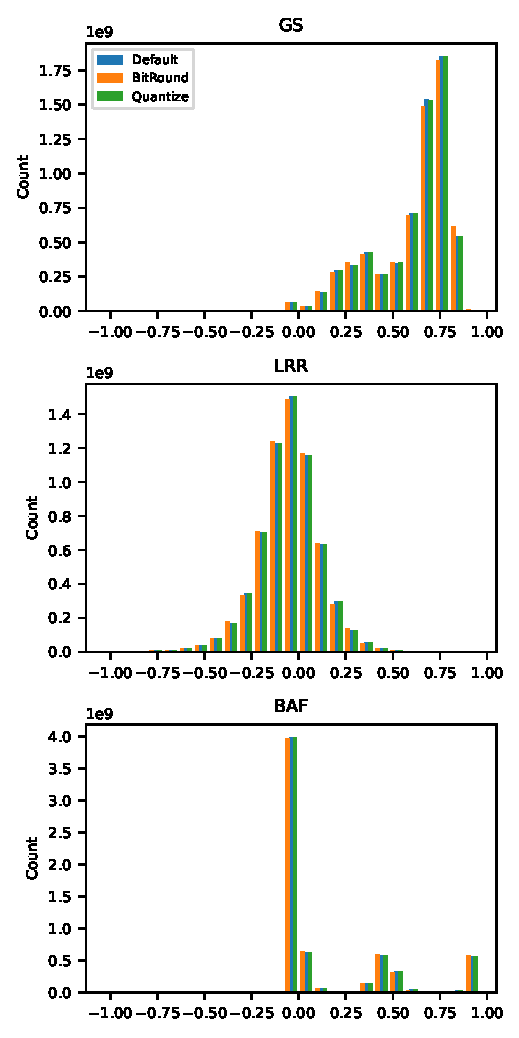
\includegraphics{figures/ofh-histograms}
\caption{Distribution of values in the GS, LRR and BAF fields in the Our Future
Health data with no truncation (Default), and truncation using the BitRound
and Quantize filters.
\label{fig-ofh-field-distributions}}
\end{figure}

\begin{figure}[h]
\includegraphics{figures/compression-compressor}
\caption{Effects of Blosc compression codec on compression ratio on call-level
fields in 1000 Genomes data.
In all cases compression level=7 was used, with a variant
chunk size of 10,000 and sample chunk size of 1,000.
Bit shuffle was used for call\_genotype, and no shuffle used for the other fields.
\label{fig-compression-compressor}}
\end{figure}

\begin{figure}[h]
\includegraphics{figures/compression-shuffle}
\caption{Effects of Blosc shuffle settings on compression ratio on call-level
fields in 1000 Genomes data.
In all cases the zstd compressor with compression level=7 was used, with a variant
chunk size of 10,000 and sample chunk size of 1,000.
\label{fig-compression-shuffle}}
\end{figure}

\begin{figure}[h]
\includegraphics{figures/compression-chunksize}
\caption{Effects of chunk sizes on compression ratio on call-level
fields in 1000 Genomes data.
(A) Varying sample chunk size, holding variant chunk size fixed at 10,000.
(B) Varying variant chunk size, holding sample chunk size fixed at 1,000.
In all cases the zstd compressor with compression level=7 was used. Bit shuffle
was used for call\_genotype, and no shuffle used for the other fields.
Values are chosen to be evenly spaced on a linear scale
between 100 and 2504 (the number of samples) in (A) and
evenly spaced between 100 and 96514 on a log scale in (B).
\label{fig-compression-chunksize}}
\end{figure}

\begin{figure}[h]
\includegraphics{figures/compression-chunksize-finegrained.pdf}
\caption{Effects of sample chunk size on compression ratio on the call\_genotype
field in 1000 Genomes data.
The same analysis as in Fig~\ref{fig-compression-chunksize}, except we only
consider call\_genotype and we examine all sample chunk sizes from
100 to 256. Distinct trend-lines emerge for odd, even and multiple-of-four
chunk sizes (shown by markers). The size of the final chunk also has a minor
effect (shown by colour).
\label{fig-compression-chunksize-finegrained}}
\end{figure}

\end{document}
